\documentclass[11pt]{book}
\usepackage{graphicx}
\DeclareGraphicsRule{.tiff}{png}{.png}{`convert #1 `dirname #1`/`basename #1 .tiff`.png}

\usepackage{amsmath,amssymb}
\usepackage{times}
\usepackage{epstopdf}
\usepackage[ligature,reserved]{semantic}
\usepackage[center,tight]{subfigure}
\usepackage{proof}

\usepackage{color}

\definecolor{red}{rgb}{1,0,0}
\definecolor{magenta}{cmyk}{0,1,0,0}
\definecolor{halfgrey}{gray}{0.5}

\textwidth = 6.5 in
\textheight = 9 in
\oddsidemargin = 0.0 in
\evensidemargin = 0.0 in
\topmargin = 0.0 in
%\headheight = 0.0 in
%\headsep = 0.0 in
\parskip = 3pt
\parindent = 0.0in

%no indent on footnotes
\makeatletter
\renewcommand{\@makefntext}[1]{\setlength{\parindent}{0pt}%
\begin{list}{}{\setlength{\labelwidth}{1em}%
  \setlength{\leftmargin}{\labelwidth}%
  \setlength{\labelsep}{3pt}\setlength{\itemsep}{0pt}%
  \setlength{\parsep}{0pt}\setlength{\topsep}{0pt}%
  \footnotesize}\item[\hfill\@makefnmark]#1%
\end{list}}
\makeatother

%\newtheorem{theorem}{Theorem}
%\newtheorem{corollary}[theorem]{Corollary}
%\newtheorem{definition}{Definition}

\title{\huge Natural Deduction Proof and Disproof in Jape}
\author{Richard Bornat (richard@bornat.me.uk)}

\mathlig{->}{\rightarrow}
\mathlig{|-}{\vdash}
\mathlig{|=}{\vDash}
\mathlig{|*}{\exists}
\mathlig{|}{\lor}
\mathlig{!}{\neg}
\mathlig{@*}{\forall}
\mathlig{@}{\land}

\reservestyle{\word}{\operatorname}
\word{actual}

\reservestyle{\var}{\mathit}
\var{j1,j2}

\newcommand{\eqnref}[1]{(\ref{eqn:#1})}
\newcommand{\figref}[1]{figure \ref{fig:#1}}
\newcommand{\Figref}[1]{Figure \ref{fig:#1}}
\newcommand{\secref}[1]{section \ref{sec:#1}}
\newcommand{\Secref}[1]{Section \ref{sec:#1}}
\newcommand{\chapref}[1]{chapter \ref{chap:#1}}
\newcommand{\Chapref}[1]{Chapter \ref{chap:#1}}

\begin{document}
\maketitle


\chapter*{Preface}

This manual is a how-to for Jape and my Natural Deduction encoding. Earlier versions contained a good deal of logic teaching. That's been dropped, since now there's a book (Logic for Programmers, OUP) which says it all a good deal better. You will learn about logic by playing with Jape, so I suppose there's still teaching in there.

This document was written on a Mac, and the illustrations are all taken from the MacOS X version of Jape. All Japes, on Linux, Solaris, Windows, MacOS X or whereever, run exactly the same code but the interfaces can look slightly different. I haven't produced different versions of the manual because I think --- rather, I hope --- that those differences in fonts, in window controls, in the placing of menus and so on, don't really matter. If I'm wrong then I hope somebody will tell me.

\section*{Jape or NDJape?}

This manual is really about how Jape, which is capable of working with many different logics, has been made to deal with Natural Deduction as described in my book. Instead of talking about what `Jape' does when dealing with $->$ formulae, I should really talk about what `Jape loaded with the I2L encoding' does. But that's such a mouthful that I just talk as if there is only one Jape, and all it does is Natural Deduction.

If you're interested there's a manual on the website (http://www.japeforall.org.uk) which tells you how to roll your own logic encodings. Best of luck.

\section*{Differences from the book}
\begin{itemize}
\item Jape writes its premises on a single line, separated by commas, instead of using a separate line for each premise;
\item Jape writes quantifications as $@*x.P(x)$ and $|*y.Q(y)$ --- with a dot between bound variable and predicate --- instead of $@*x(P(x))$ and $|*y(Q(y))$
\end{itemize}
So far as I know, these are the only significant differences.

\section*{Any comments?}

If Jape doesn't work for you, it isn't working, and if it isn't working I'd like to hear about it. 

Please send any comments, thoughts, complaints or whatever to me (see title page for email address). I'll do my best to reply quickly and if your message is of general interest I'll put it up on the website (with your permission, and hiding your email address from the spambots at least). 

\section*{Acknowledgements}

I designed and built Jape between 1991 and 2002 whilst I was at Queen Mary College, University of London, working with Bernard Sufrin of the Bernard Sufrin of the Computer Laboratory, Oxford University. I've continued to develop it at Middlesex University since. Bernard worked on the implementation with me for the first four years or so. That doesn't describe all he did: his design insights were crucial and without him Jape wouldn't exist or be half as good as it is. His program architecture, which he worked out in the first few months of our collaboration, is still in place even though Jape has been rebuilt from the ground up more than once. He still produces the Jape distributions and running the www.japeforall.org.uk website.

For the rest of it I've been strongly influenced by colleagues at Queen Mary, many of whom have made seminal suggestions which have improved Jape. In alphabetical order I single out Jules Bean, John Bell, Peter Burton, Keith Clarke, Adam Eppendahl, David Pym, Graem Ringwood, Mike Samuels, Paul Taylor and Graham White. 

Jape began as an experiment towards the end of an EPSRC research project on the use of symbolic calculators to teach formal reasoning, joint with Steve Reeves and Doug Goldson at Queen Mary, and Tim O'Shea and Pat Fung at the Open University. A later project, with Pat Fung and James Aczel from the OU, looked at students using Jape; James's insightful summary of their difficulties led to a redesign of the treatment of natural deduction, and directly to this version of the program.

Jape's proof engine was originally written in SML and compiled by SMLNJ, with interfaces for different operating systems written in C, tcl/tk, Python and I can't remember what else. In 2002 I ported the engine to OCaml and wrote a system-independent interface module in Java. I'm grateful to the implementers of all those languages, especially for their decision to provide their software for free. Jape is free too, at http:www.japeforall.org.uk. 

\tableofcontents

\chapter{Basics}


\begin{figure}
\centering
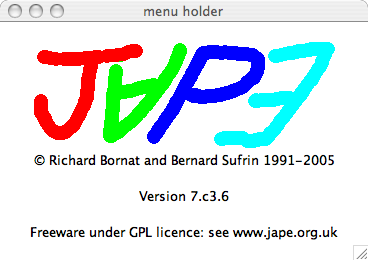
\includegraphics[scale=0.5]{pics/splashscreen.png}
\caption{The Jape splash screen}
\label{fig:splashscreen}
\end{figure}
\begin{figure}
\centering
\parbox[b]{165pt}{\centering
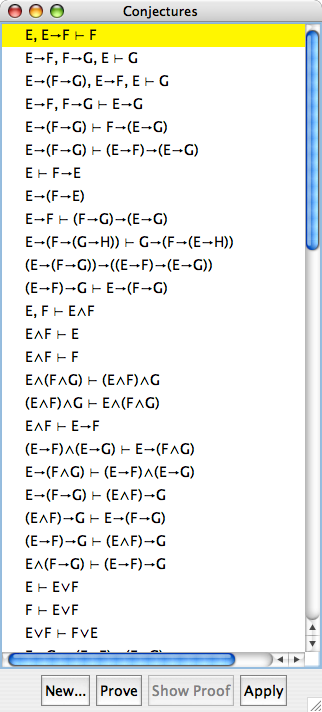
\includegraphics[scale=0.5]{pics/conjecturespanel.png}
\caption{The Conjectures panel}
\label{fig:conjecturespanel}}
\qquad
\parbox[b]{230pt}{\centering
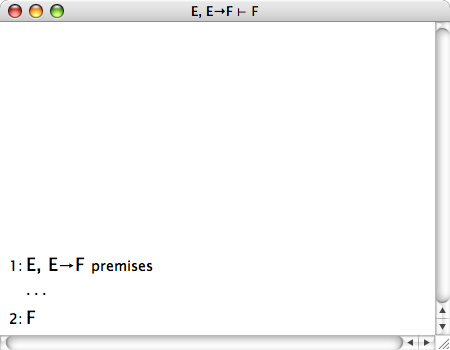
\includegraphics[scale=0.5]{pics/firstproofwindow.png}
\caption{A proof window}
\label{fig:firstproofwindow}}
\end{figure}

\section{Getting started}

If you don't already have Jape, download it from http://www.japeforall.org.uk. Install it, following the instructions carefully.

You should have a directory containing the Jape application and a subdirectory called examples. Double-click Jape, and you will see a window like \figref{splashscreen}.\footnote{You may see minor differences. The illustrations in this manual are taken from MacOS X. On Windows and Linux you will see a menu bar in the window and the window title will be Jape. But those differences don't matter much, so I won't refer to them again.}

Using the Open New Theory command in  the File menu, open examples/natural\_deduction/I2L.jt. You should see several windows containing logical conjectures (claims to be proved), called \emph{panels} in Jape. The Conjectures panel should look something like \figref{conjecturespanel} (you will probably have to resize the window to make it look like this). Double-click any line to begin, or select a line and press the Prove button at the bottom of the panel. You will see a \emph{proof window} like \figref{firstproofwindow}, and off you go!

\begin{figure}
\centering
\parbox[b]{200pt}{\centering
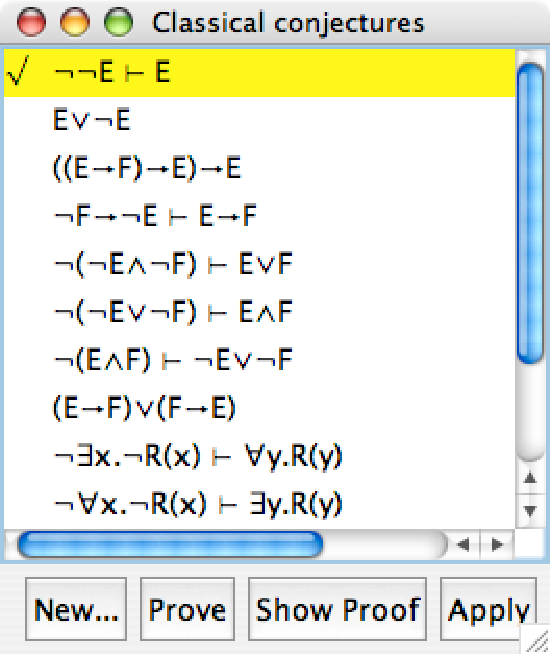
\includegraphics[scale=0.5]{pics/provedconjecture}
\caption{A conjecture panel with a proved conjecture}
\label{fig:provedconjecture}}
\qquad
\parbox[b]{200pt}{\centering
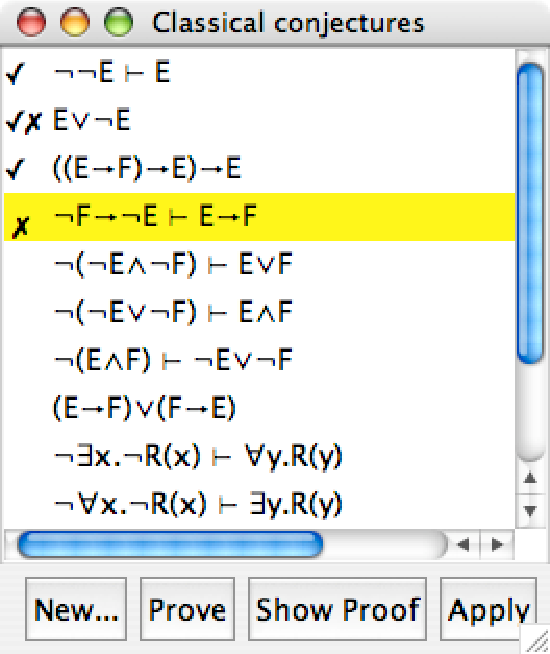
\includegraphics[scale=0.5]{pics/decoratedpanel}
\caption{A conjecture panel with proved and disproved conjectures}
\label{fig:decoratedpanel}}
\end{figure}

\section{Finishing a proof}

When you have made a proof of a conjecture --- no more lines of dots in the proof window --- you can save it: pull down the Edit menu and select Done. The proof window closes, and Jape records the fact that the conjecture is proved, marking its entry in the conjectures panel with a tick in the margin, as illustrated in \figref{provedconjecture}. If you disprove a conjecture (see \chapref{disproof}) then you can record that too, and you get a cross in the margin. Because classical proof and constructive disproof overlap, you can even get both marks against the same conjecture, as illustrated in \figref{decoratedpanel}.

Proof of a conjecture makes it a theorem. You can use theorems in your proofs as if they were additional Natural Deduction rules (select the theorem in the panel, press the Apply button), and you can review their proofs using the Show Proof button. See \chapref{theorems} for more information.

\section{Saving and restoring your work}

Jape offers to record your proofs --- saved and unsaved --- when you quit or when you choose ``Save Proofs'' or ``Save Proofs As ...'' from the File menu. It will reload saved proofs using ``Open ...'', also from the File menu. 

\section{Printing and Exporting}

You can print a proof using the Print Proof command on the Edit menu. If you have a disproof on the go (see \chapref{disproof}) you can print it using the Print Disproof command, or proof and disproof together using Print. 

To make a pdf or ps copy of a proof in a file, use Export Proof, Export Disproof or Export, all on the Edit menu.

\section{Making Jape work for you}

\subsection{Only reflect}

Jape is designed to be easy to use, which means that the mouse and menu and window stuff don't get in the way of the logic. It's so easy to use that you can have great fun clicking away, `solving' lots of problems without always knowing exactly what you're doing. That's ok, because you can learn while you're having fun, and you can do things for yourself without asking for help. But it's obviously not the whole story.

Because Jape is easy to use it brings you quickly to a point where you can ask interesting and important questions. The kind of question you are supposed to ask is ``is the logic really supposed to work like \emph{that}?'' If there are experts around you can ask them, but if you are on your own you can still ask yourself. That isn't a daft thing to do: educationalists call it \emph{reflection}, and it's one of the best ways to learn.

Some logical proofs are hard to believe at first. Some single logical steps are pretty surprising. I hope that you will always read through finished Jape proofs to see if you can believe them. If there is a surprise, ask yourself: where does the surprise come from? By undoing and redoing steps you can watch the surprise emerge and explain to yourself why it's necessary.

Jape's a machine, and that has disadvantages as well as advantages. The big advantage is that a machine can do formal calculation --- proof and disproof --- perfectly, without mistake. The big disadvantage is that it can't understand anything about what it's doing. Jape doesn't know the difference between a nice proof and a nasty one. Sometimes reflection will show you that there is a shorter or prettier proof than the one you have made. You can always undo your work and try again!

\subsection{Be brave}

We read proofs top-to-bottom most of the time. Novices, reasonably but mistakenly, imagine that proofs are constructed top-to-bottom too: start at line 1 and work forwards. Well, sometimes it is done that way, but at least as often it's done the other way round, bottom-to-top, starting with the last line and working backwards. Be brave and try it! If you stick to forward proof you make life very difficult for yourself, so bravery pays dividends.

Bravery is needed, too, when learning how proof steps work. It's reasonable when playing with an interactive program to first try only steps that make small changes, but eventually you have to try everything. It's just like riding a bike: once you've plucked up courage you can't remember what it felt like to be scared of $|$ elim or $@$ intro or whatever. Just do it!  

\subsection{Never guess an assumption}

A proof is really a \emph{structure of deductions}, not a sequence of lines, and its assumption boxes show that structure. Reading a proof from top to bottom, every assumption that is introduced must also be \emph{discharged} by the use of a rule which makes use of the box. Jape guarantees correct use of assumptions by combining introduction and discharge into a single step. Assumptions are introduced (and discharged) by using rules, and the rules that do it --- some forward, some backward --- are labelled in the menus. Jape helps you, in every case, by calculating the assumption that you need: there is \emph{never} a need to guess an assumption.

\chapter{Gestures: mouse clicks, presses and drags}
\label{chap:gestures}

Like every other interactive program, Jape accepts instructions through the mouse and the keyboard. Mostly you will use the mouse to \emph{select} a formula or a subformula in the proof window and then to \emph{command} what to do with your selection by choosing a command from a menu. The ways that Jape uses the mouse are pretty standard.

\begin{figure}
\centering
\subfigure[hypothesis selection]{
  \label{fig:hypothesisselection}
  \parbox[b]{100pt}{\centering\fbox{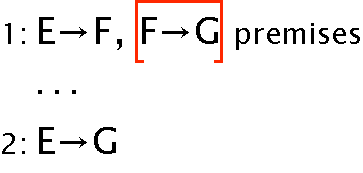
\includegraphics[scale=0.5]{pics/hypothesisselection}}}}
\quad
\subfigure[conclusion selection]{
  \label{fig:conclusionselection}
  \parbox[b]{100pt}{\centering\fbox{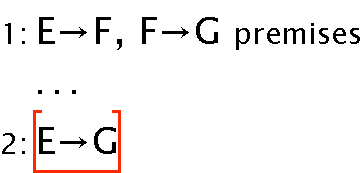
\includegraphics[scale=0.5]{pics/conclusionselection}}}}
\quad
\subfigure[hypothesis and conclusion]{
  \label{fig:hypothesisandconclusion}
  \parbox[b]{100pt}{\centering\fbox{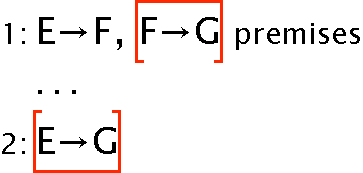
\includegraphics[scale=0.5]{pics/hypothesisandconclusion}}}}
\quad
\subfigure[multi-hypothesis selection]{
  \label{fig:multipleselection}
  \parbox[b]{100pt}{\centering\fbox{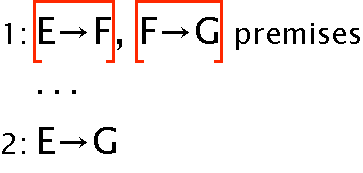
\includegraphics[scale=0.5]{pics/multipleselection}}}}
\caption{Formula selection by mouse click}
\end{figure}

\section{Formula selection}
\label{sec:formulaselection}

Formula selection is made with a single click (left-click on a multi-button mouse). You click on a formula --- a \emph{hypothesis} above the line of dots or a \emph{conclusion} below the dots --- and Jape highlights your selection with an enclosing red box. If you click on a hypothesis you get a downward-facing box as in \figref{hypothesisselection}; if you click on a conclusion you get an upward-facing box as in \figref{conclusionselection}. You can select both a hypothesis and a conclusion, as in \figref{hypothesisandconclusion}.

Clicking on the background --- a white part of the proof window --- cancels all your selections.

Simple clicks will let you select one conclusion and one hypothesis at a time. Normally a second hypothesis click cancels the first, but if you hold down the Shift key while you click you can select more than one hypothesis, as shown in \figref{multipleselection}. And then, also using the Shift key whilst clicking, you can cancel individual formula selections.

There is no way of selecting more than one conclusion at a time.

\begin{figure}
\centering
\subfigure[Proof attempt with intermediate hypothesis/conclusion formula]{
  \label{fig:ambiguousformula}
  \parbox[b]{130pt}{\centering\fbox{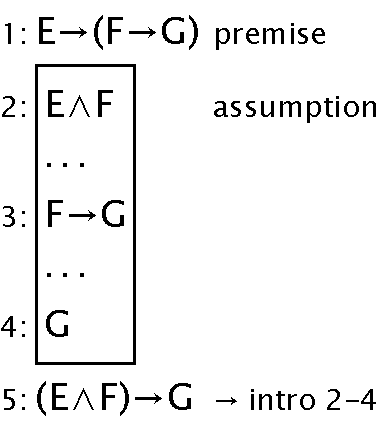
\includegraphics[scale=0.5]{pics/ambiguousformula}}}}
\quad
\subfigure[top-half click selects as conclusion]{
  \label{fig:ambiguousconclusion}
  \parbox[b]{130pt}{\centering\fbox{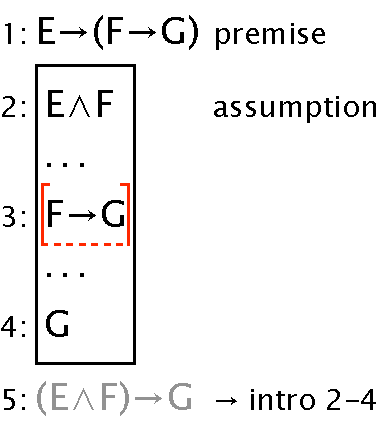
\includegraphics[scale=0.5]{pics/ambiguousconclusion}}}}
\quad
\subfigure[bottom-half click selects as hypothesis]{
  \label{fig:ambiguoushypothesis}
  \parbox[b]{130pt}{\centering\fbox{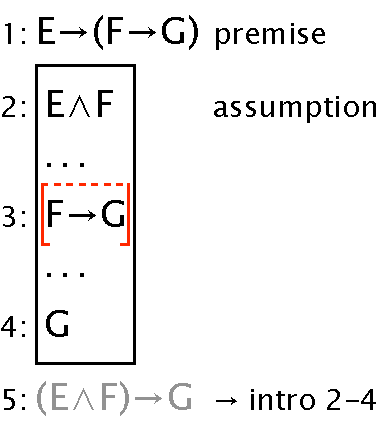
\includegraphics[scale=0.5]{pics/ambiguoushypothesis}}}}
\caption{Ambiguous conclusion/hypothesis selection}
\end{figure}

\subsection{Ambiguous formulae click both ways}

In \figref{ambiguousformula} there are open conclusions on lines 3 and 4, each preceded by a line of dots to show that there's work to be done. Lines 1 and 2 aren't conclusions, and can only be used as hypotheses to prove lines 3 and 4. Line 5 can't be used at all: it's a proved conclusion. Line 4 can only be a conclusion and not a hypothesis, because there's nothing below it in the box. But line 3 is ambiguous: it has to be proved as a conclusion, perhaps using lines 1 and 2, and it can be used as a hypothesis to prove line 4. 

Ambiguous formulae like $F->G$ on line 3 of \figref{ambiguousformula} can be selected in two ways. If you click on the \emph{top half} of the formula you get a box open at the top --- i.e. a conclusion selection --- with a dotted line across the bottom, as shown in \figref{ambiguousconclusion}. If you click on the \emph{bottom half} you get a box open at the bottom --- i.e. a hypothesis selection --- with a dotted line across the top, as shown in \figref{ambiguoushypothesis}.

\subsection{Greying-out}

When you select a hypothesis you can only make a step towards conclusions below you and in the same box as the hypothesis you clicked. When you select a conclusion you can only make a backward step towards hypotheses above you and in the same box or enclosing boxes. Jape greys out all the formulae you can't use, to help you see what's going on, as shown by line 5 in figures \ref{fig:ambiguousconclusion} and \ref{fig:ambiguoushypothesis}. 

If you click on a greyed-out formula Jape cancels your current selection(s). If you click on a conclusion that's already been used up (one which isn't immediately below a line of dots) then Jape greys it out and cancels all your selections.\footnote{This was once a bug. Now it's become a feature, because I rather like it.}

\begin{figure}
\centering
\subfigure[subformula selection]{
  \label{fig:singlesubformulaselection}
  \parbox[b]{150pt}{\centering\fbox{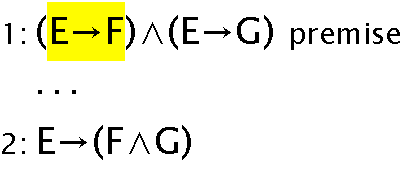
\includegraphics[scale=0.5]{pics/singlesubformulaselection}}}}
\quad
\subfigure[multiple-subformula selection]{
  \label{fig:multiplesubformulaselection}
  \parbox[b]{150pt}{\centering\fbox{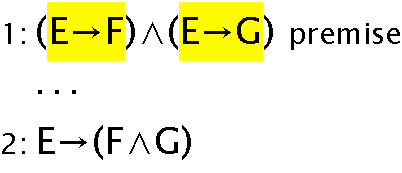
\includegraphics[scale=0.5]{pics/multiplesubformulaselection}}}}

\caption{Subformula selection by option/alt/middle-press-and-drag}
\end{figure}

\section{Subformula selection}
\label{sec:subformulaselection}

Occasionally you need to tell Jape to focus on part of a formula. You do this by a press-and-drag gesture:
\begin{itemize}
\item with a three-button mouse, middle-press-and-drag;
\item otherwise by holding the Alt shift (sometimes labelled 'option') during a press-and-drag.
\end{itemize}

Jape highlights the subformula you've selected by changing the background colour to yellow, as shown in \figref{singlesubformulaselection}. 

If you hold down the add-a-selection key (ctrl on Windows and Linux, command on MacOS X) you can make more than one subformula selection, as shown in \figref{multiplesubformulaselection}. Using the same key combination, you can cancel and/or modify subformula selections you've already made.

Jape restricts subformula selections to well-formed subformulae, as you can discover by experiment. That means that if you option/alt/middle-click on a connective or a quantifier, a whole subformula is highlighted. If you option/alt/middle-click on a name, only that name is highlighted.

Option/alt/middle-clicking or pressing on a new subformula cancels all other subformula selections, unless you hold down the add-a-selection key (Command on MacOS, Ctrl on other systems). Option/alt/middle-clicking on the background --- a white part of the proof window --- cancels all your subformula selections.

Formula and subformula selections are independent: you can have one without the other, or both, or neither. Cancelling one kind of selection doesn't cancel the other. 

\section{Dragging}

In the disproof pane --- see \chapref{disproof} --- you can drag formulae, tiles, worlds and lines around to make a diagram. You do it by press-and-drag. See \chapref{disproof} for details.


\chapter{Backward and forward steps}
\begin{figure}
\centering
\parbox[b]{200pt}{\centering
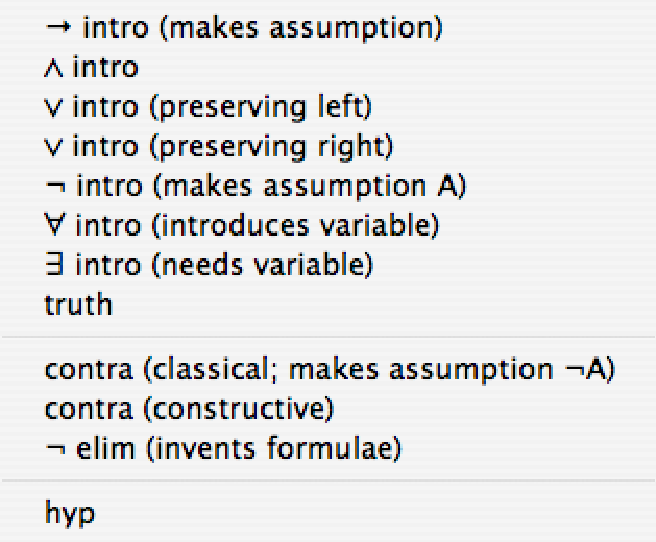
\includegraphics[scale=0.6]{pics/backwardmenu}
\caption{Backward menu}
\label{fig:backwardmenu}}
\qquad
\parbox[b]{200pt}{\centering
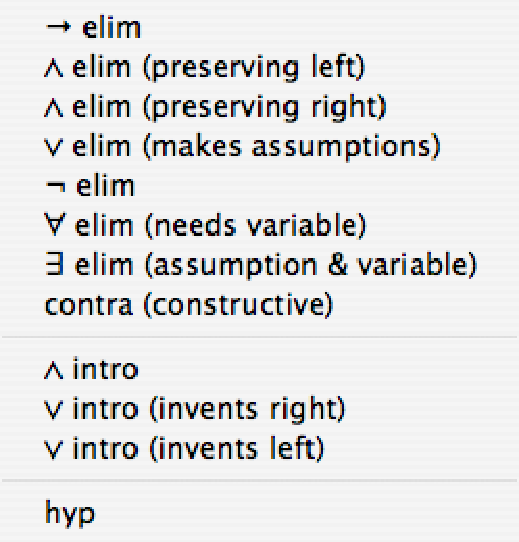
\includegraphics[scale=0.6]{pics/forwardmenu}
\caption{Forward menu}
\label{fig:forwardmenu}}
\end{figure}

Because we read proofs forward, top-to-bottom, forward steps are easiest to understand and most proof novices prefer working forwards. But lots of proofs are difficult working forwards, and some are almost impossibly difficult. To make proofs in Jape you need to be able to make backward steps as well, and I've gone to some trouble to force you to recognise the fact. In the Backward menu, shown in \figref{backwardmenu}, the first group of steps above the line work best backwards and the group below that line can be made to work backward if you try hard. The Forward menu, in \figref{forwardmenu}, similarly shows steps that work well forward before ones that work forward only with difficulty. `hyp' is hard to classify, so it appears in both menus.

To make a step you select one or more formulae and choose a step from the Backward or Forward menu. The selections you need to make depend on the step you choose, and are detailed in the descriptions of the steps in later chapters, but in general for a forward step you must choose a hypothesis and for a backward step an open (unproved) conclusion.

\begin{figure}
\centering
\subfigure[before]{
  \label{fig:two-selectionforwardstepbefore}
  \parbox[b]{200pt}{\centering\fbox{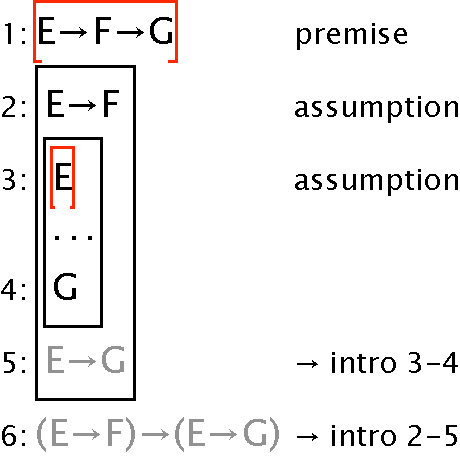
\includegraphics[scale=0.5]{pics/two-selectionforwardstepbefore}}}}
\qquad
\subfigure[after]{
  \label{fig:two-selectionforwardstepafter}
  \parbox[b]{200pt}{\centering\fbox{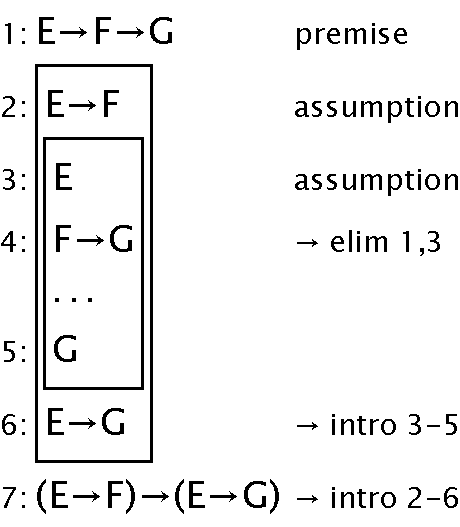
\includegraphics[scale=0.5]{pics/two-selectionforwardstepafter}}}}
\caption{A sample forward step}
\label{fig:two-selectionforwardstep}
\end{figure}
\section{Making a forward step}

Before you make a forward step you must always select a hypothesis formula. Depending on the kind of step, you may have to select more than one hypothesis: for details, see the description of the step later in this manual --- or just try it and see what happens!

You can also select a conclusion as well, if you want to. Some steps require a conclusion selection: you can look up the step in this manual or you can try it out and see what happens. 

Once you have made your selection(s), choose your step from the Forward menu.

Jape writes the result of the step --- the consequent deduced from the antecedent(s) you selected --- just below your selection(s). For example, \figref{two-selectionforwardstep} shows an $->$ elim step with two hypothesis selections. The consequent is line 4 in the `after' picture. Notice that the justification of the step is written against the consequent.

\begin{figure}
\centering
\subfigure[hypothesis only selected]{
  \label{fig:hypselectedignoringtargetbefore}
  \parbox[b]{200pt}{\centering\fbox{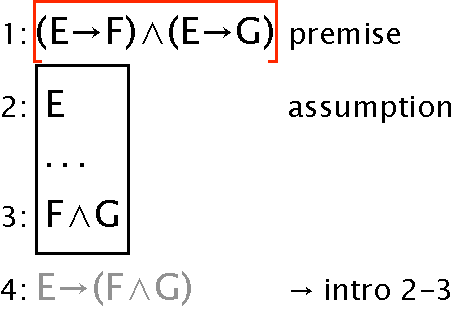
\includegraphics[scale=0.5]{pics/hypselectedignoringtargetbefore}}}}
\qquad
\subfigure[consequent below hypothesis]{
  \label{fig:hypselectedignoringtargetafter}
  \parbox[b]{200pt}{\centering\fbox{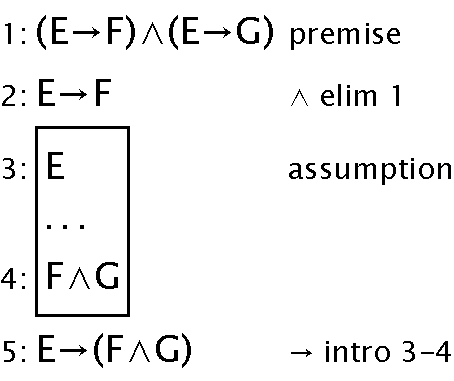
\includegraphics[scale=0.5]{pics/hypselectedignoringtargetafter}}}}
\caption{A forward step without a target conclusion}
\label{fig:hypselectedignoringtarget}
\end{figure}
\begin{figure}
\centering
\subfigure[hypothesis and conclusion selected]{
  \label{fig:hypselectedwithtargetbefore}
  \parbox[b]{200pt}{\centering\fbox{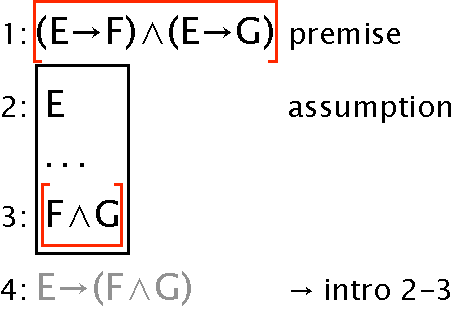
\includegraphics[scale=0.5]{pics/hypselectedwithtargetbefore}}}}
\qquad
\subfigure[consequent above conclusion]{
  \label{fig:hypselectedwithtargetafter}
  \parbox[b]{200pt}{\centering\fbox{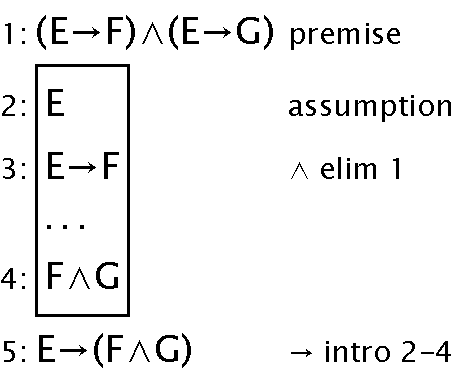
\includegraphics[scale=0.5]{pics/hypselectedwithtargetafter}}}}
\caption{A forward step with a target conclusion}
\label{fig:hypselectedwithtarget}
\end{figure}

\subsection{Selecting a target conclusion}

Normally Jape writes the result of a forward step just after 
the hypothesis selection. Sometimes that may not be convenient, 
and it may be tidier to write it lower down the proof, just above 
a conclusion you are working towards.

In \figref{hypselectedignoringtargetbefore} only the hypothesis on line 1 is selected. A forward step --- in this case ``$@$ elim (ignoring right)'' --- puts its consequent just below the selected hypothesis, as shown in \figref{hypselectedignoringtargetafter}.

If you select a target conclusion as well, as in \figref{hypselectedwithtargetbefore}, the same step will put its consequent before the line of dots above the selected conclusion, as shown in \figref{hypselectedwithtargetafter}.

\subsection{What can go wrong with a forward step?}

When Jape can't make a forward step it's for one of the following reasons. In all cases you'll get an error message which explains the problem.
\begin{enumerate}
\item \emph{No selected hypothesis}. \\
If you don't select a hypothesis formula, you can't make a forward step.

\item \emph{Not enough selections}.\\
Some steps need more than a single hypothesis selection. 

\item \emph{Wrong hypothesis shape}.\\
Most forward steps apply to a particular shape of hypothesis formula. If you select the wrong shape, you can't make the step.

\begin{figure}
\centering
\subfigure[before: hypothesis and conclusion selected]{
  \label{fig:velimneedstargetconclusionbefore}
  \parbox[b]{200pt}{\centering\fbox{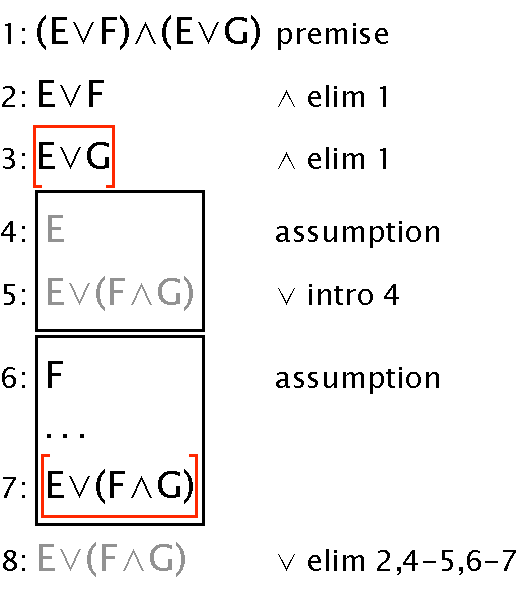
\includegraphics[scale=0.5]{pics/velimneedstargetconclusionbefore}}}}
\qquad
\subfigure[after: argument by cases outlined]{
  \label{fig:velimneedstargetconclusionafter}
  \parbox[b]{200pt}{\centering\fbox{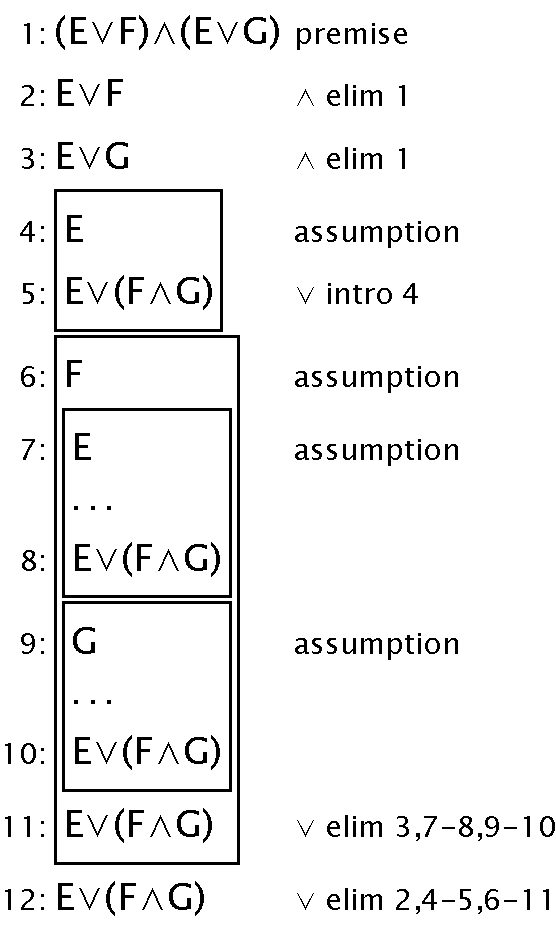
\includegraphics[scale=0.5]{pics/velimneedstargetconclusionafter}}}}
\caption{$|$ elim needs a target conclusion}
\label{fig:velimneedstargetconclusion}
\end{figure}

\item \emph{No target conclusion}.\\
Two forward steps --- $|$ elim, $|*$ elim --- need a conclusion selection as well as a hypothesis, because the consequent can't be calculated from the antecedents. Jape writes the result of the step just above the target conclusion, and writes the justification next to the selected consequent. For example, see the $|$ elim step 
in \figref{velimneedstargetconclusion}. The result of the step (there's quite a lot of it!) is written above line 7 of the `before' state, to form lines 7 to 10 of the `after' state.

%\item \emph{Nowhere to go}.

%When you select a hypothesis, Jape greys-out all the open (unproved) 
%conclusions except the ones that can make use of the hypothesis. 
%If there aren't any reachable open conclusions, Jape won't let you make 
%the forward step (because what use could you make of the result?). 
%In \figref{forwardstepnotarget} there are no open conclusions which can make 
%use of line 2 (there is an open conclusion on line 8, but it's greyed-out because 
%it is in another box and line 2 is irrelevant to it).

%\begin{figure}
%\begin{center}
%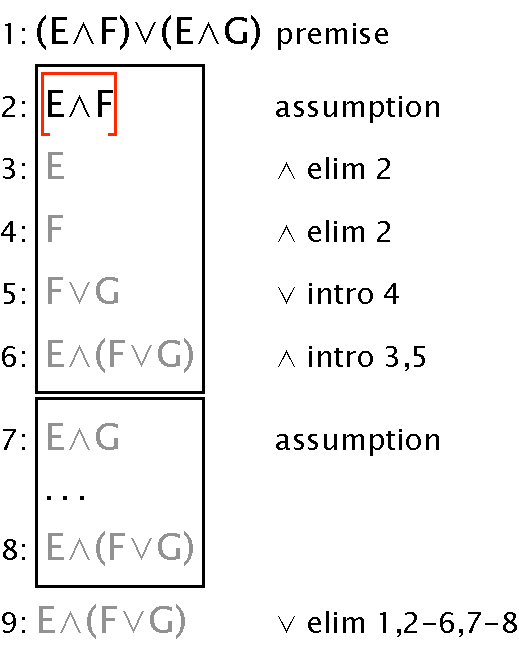
\includegraphics[scale=0.5]{pics/forwardstepnotarget}
%\caption{Hypothesis selection with no open conclusion}
%\label{fig:forwardstepnotarget}
%\end{center}
%\end{figure}

\end{enumerate}



\begin{figure}
\centering
\subfigure[conclusion selected]{
  \label{fig:concselectedforbackwardstep}
  \parbox[b]{200pt}{\centering\fbox{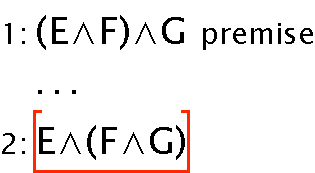
\includegraphics[scale=0.5]{pics/concselectedforbackwardstep}}}}
\qquad
\subfigure[two new conclusion antecedents]{
  \label{fig:concselectedforbackwardstepresult}
  \parbox[b]{200pt}{\centering\fbox{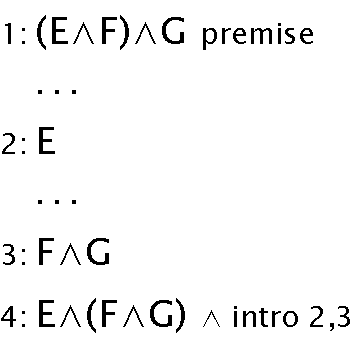
\includegraphics[scale=0.5]{pics/concselectedforbackwardstepresult}}}}
\caption{A sample backward step}
\label{fig:samplebackwardstep}
\end{figure}
\begin{figure}
\centering
\subfigure[conclusion selected]{
  \label{fig:concselectedforbackwardstep2}
  \parbox[b]{200pt}{\centering\fbox{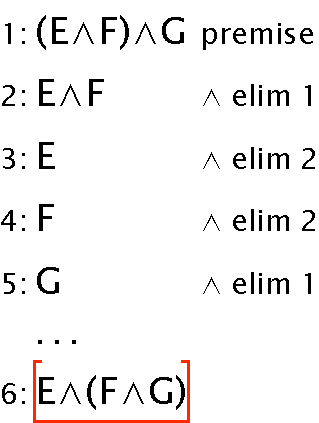
\includegraphics[scale=0.5]{pics/concselectedforbackwardstep2}}}}
\qquad
\subfigure[one hypothesis, one conclusion antecedent]{
  \label{fig:concselectedforbackwardstep2result}
  \parbox[b]{200pt}{\centering\fbox{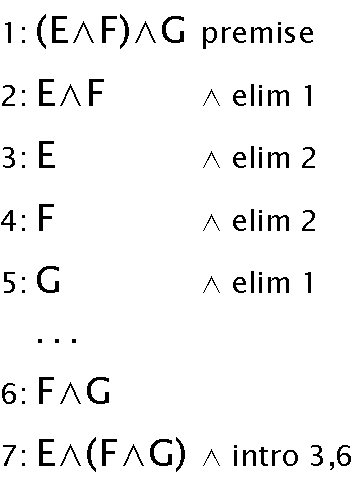
\includegraphics[scale=0.5]{pics/concselectedforbackwardstep2result}}}}
\caption{A sample backward step with a relevant hypothesis}
\label{fig:samplebackwardstepwithhyp}
\end{figure}

\section{Making a backward step}

Backward steps work on an open conclusion --- a line without a justification, written just below a line of three dots. They may prove it completely, if Jape can find hypotheses to match the antecedents, or the antecedents may become unproved conclusions. For example, \figref{concselectedforbackwardstep} shows an open conclusion selection, and \figref{concselectedforbackwardstepresult} shows the effect of a backward $@$ intro step, where each antecedent has become a new open conclusion. \Figref{concselectedforbackwardstep2} shows the same conclusion selected when there are more hypothesis formulae available, and in \figref{concselectedforbackwardstep2result} only one open conclusion is generated because line 3 matches the antecedent of the $@$ intro step.

In every case the justification of the step is written next to the selected conclusion, the consequent of the step.

\subsection{What can go wrong with a backward step?}

\begin{enumerate}
\item \emph{Wrong conclusion shape}.\\

Each backward step, except for contra, applies to a particular shape of consequent formula. If you select the wrong shape, you  can't make the step.

\begin{figure}
\centering
\subfigure[$E$ is the consequent]{
  \label{fig:concselectiondisambiguatesA}
  \parbox[b]{200pt}{\centering\fbox{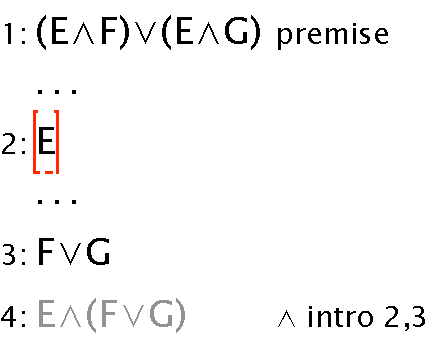
\includegraphics[scale=0.5]{pics/concselectiondisambiguatesA}}}}
\qquad
\subfigure[$F|G$ is the consequent]{
  \label{fig:concselectiondisambiguatesB}
  \parbox[b]{200pt}{\centering\fbox{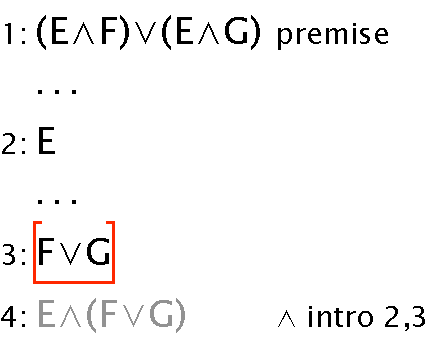
\includegraphics[scale=0.5]{pics/concselectiondisambiguatesB}}}}
\caption{Conclusion selection to tell Jape where to work}
\label{fig:concselectiondisambiguates}
\end{figure}

\item \emph{No selected consequent.}\\
If there is more than one unproved conclusion, Jape doesn't try to choose between them. In \figref{concselectedforbackwardstepresult}, for example, Jape wouldn't know where to apply a backward step. Selecting an unproved conclusion, as in \figref{concselectiondisambiguates}, resolves the ambiguity. (Notice in \figref{concselectiondisambiguatesA} that line 2 is an ambiguous hypothesis/conclusion formula, selected as a conclusion by clicking on it's top half.)\\

\item \emph{Hypothesis selected}.\\
Backward steps (except for $|*$ intro) don't need and can't make use of a selected hypothesis formula. 

\end{enumerate}

\section{Steps which don't need a selection}

If there is only one formula in the proof that can be selected 
as a hypothesis, it would be annoying to be told to select it 
before you can make a forward step. If there's only one unproved 
conclusion in the proof, it would be annoying to be told to select 
that to make a backward step. If the only possible target conclusion 
is on the next line to the hypothesis, it would be annoying to 
be told to select it when a step needs a target. So in all those 
cases Jape lets you get away without selection, and does the 
obvious thing.


\chapter{Rules of thumb for proof search}

Rules of thumb\footnote{An inch was originally defined as the width 
of an adult male thumb, so a `rule of thumb' is an approximate 
measure, then (by punning `rule'=measurer) an approximate guide.\\
There is a Greek word `heuristic' for rule-of-thumb, but I 
prefer the old English. 

Some people object to the English phrase 
because there was once a folk tradition in England that a man 
could legally beat his wife with a stick no thicker than his 
thumb, and it was popularly called rule of thumb. (There's 
a reference, for example, in E.P. Thompson's \textit{Customs in Common}.) The tradition 
was repulsive and mistaken, but (a) it's been forgotten, 
except by historians, and (b) the `approximate guide' reading 
predates it.} are guesswork, approximate guides that don't always 
work. Proof search is much easier if you recognise some simple principles.

\begin{enumerate}
\item Almost all the rules work on the \emph{shape} of a hypothesis 
or consequent formula. Use the shape as a guide to help you choose 
a rule.

\item Use rules that introduce assumptions into the proof \emph{as 
early as possible}. Those rules are: 
\begin{itemize}
\item $->$ intro backwards (for the assumption);
\item $|$ elim forwards (for the assumptions);
\item $!$ intro backwards (for the assumption);
\item $@*$ intro backwards (for the variable);
\item $|*$ elim forwards (for the variable and the assumption).
\end{itemize}


\item $|$ intro works backwards better than it does forwards; but 
since it throws away half the conclusion you apply it to, use 
it very carefully and as late as possible.

\item $!$ elim works better forwards than it does backwards, 
once the contradictory formulae have been revealed.

\item If you use $!$ elim backwards, look for a hypothesis 
to unify with the unproved conclusion $!\_B$ (a negated 
unknown).

\item Classical contra --- `proof by contradiction' --- can be used as 
a last resort in any situation. It introduces an assumption, 
and doesn't mind what shape the consequent is. (Constructive 
contra is just as applicable, but since it doesn't introduce 
an assumption, it isn't usually much help.)

\item If Jape won't let you make the proof, you're \emph{doing it wrong}. 
There aren't any bugs in Jape's treatment of Natural Deduction, 
and all the proofs in the Conjectures and Classical conjectures 
panels are possible --- I've done them all. Similarly, all the 
ones in the Invalid conjectures panel are impossible (they are 
included so that you can disprove them --- see \chapref{disproof}).

\item Don't be afraid to Undo and Redo to search alternative routes to proof. Jape permits multiple Undos and corresponding Redos.

\end{enumerate}


\section{Look at the shape of the formula}

There is a general principle: logical steps in Natural Deduction almost always simplify a formula, removing a connective ($->$, $@$, $|$ or $!$) or a quantifier ($@*$ or $|*$) and breaking the formula into its constituent parts. Persuasion (intro) rules do that working backwards, and use (elim) rules do it forwards. To choose a rule, look for the main connective (or the quantifier) in an unproved conclusion or a hypothesis, and use the rule which works on that connective (or quantifier).

The way that rules match formulae is so nearly mechanical that I could have set Jape up to choose the relevant rule when you merely double-click on a formula. Because I want you to learn about Natural Deduction and not just the use of the mouse, I've been grandad-ish and set it up so that you have to choose the rules for yourself.

\chapter{The steps summarised}

\begin{figure}
\centering
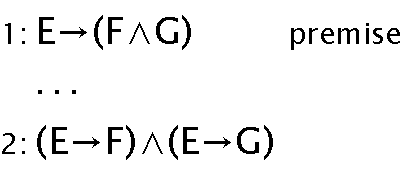
\includegraphics[scale=0.5]{pics/@introbackwardsworks}
\caption{$@$ intro backwards needed}
\label{fig:@introbackwardsworks}
\end{figure}

\section{$@$ steps}

You use $@$ intro backwards by selecting an $A@B$ conclusion and  choosing ``$@$ intro'' from the Backward menu. It generates new conclusion lines from the antecedents of the rule, as shown in figures \ref{fig:samplebackwardstep} and \ref{fig:samplebackwardstepwithhyp} on page \pageref{fig:samplebackwardstep}. I \emph{strongly recommend} using $@$ intro backwards rather than forwards.

You use $@$ elim forwards by selecting an $A->B$ hypothesis and choosing one of the two versions of the step from the Forward menu: ``$@$ elim (preserving left)'' deduces $A$, and ``$@$ elim (preserving left)'' deduces $B$. The effect is illustrated in figures \ref{fig:hypselectedignoringtarget} and \ref{fig:hypselectedwithtarget} on page \pageref{fig:hypselectedignoringtarget}.

$@$ intro forward is also possible: select two hypothesis formulae to be the antecedents and use ``$->$ intro'' from the Forward menu. But it's easier backwards, really it is. The problem in \figref{@introbackwardsworks}, for example, is easy if the first step is $@$ intro backwards --- you have two things to prove and you have to prove them separately --- and impossible almost any other way.

$@$ elim backwards is possible, but for some reason or other I didn't include it (and I'm sure I had a good reason, so I'm not going to add it now).

\begin{figure}
\centering
\subfigure[$E->(F->G)$ selected]{
  \label{fig:arrowintrobackwardbefore}
  \parbox[b]{200pt}{\centering\fbox{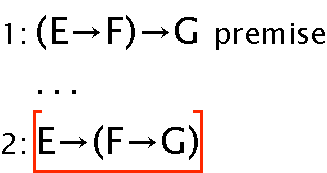
\includegraphics[scale=0.5]{pics/arrowintrobackwardbefore}}}}
\qquad
\subfigure[hypothetical argument outlined]{
  \label{fig:arrowintrobackwardafter}
  \parbox[b]{200pt}{\centering\fbox{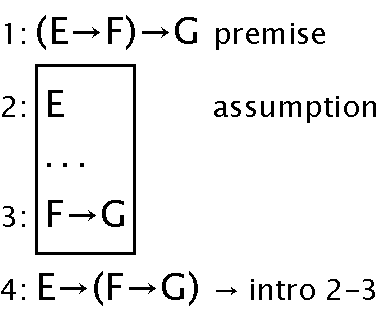
\includegraphics[scale=0.5]{pics/arrowintrobackwardafter}}}}
\caption{$->$ intro backward}
\label{fig:arrowintrobackward}
\end{figure}

\begin{figure}
\centering
\subfigure[$E$ and $E->F$ selected]{
  \label{fig:arrowelimforwardbefore}
  \parbox[b]{200pt}{\centering\fbox{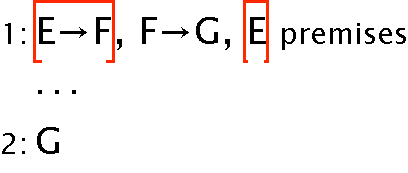
\includegraphics[scale=0.5]{pics/arrowelimforwardbefore}}}}
\qquad
\subfigure[consequent $F$ deduced]{
  \label{fig:arrowelimforwardafter}
  \parbox[b]{200pt}{\centering\fbox{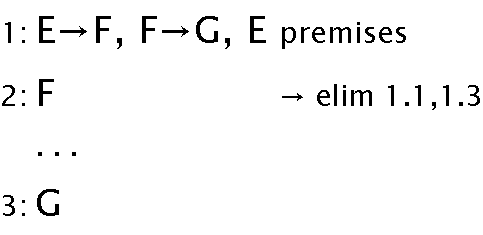
\includegraphics[scale=0.5]{pics/arrowelimforwardafter}}}}
\caption{$->$ elim forward}
\label{fig:arrowelimforward}
\end{figure}

\begin{figure}
\centering
\subfigure[$F->G$ and target conclusion selected]{
  \label{fig:-arrowelimhalfbackwardbefore}
  \parbox[b]{200pt}{\centering\fbox{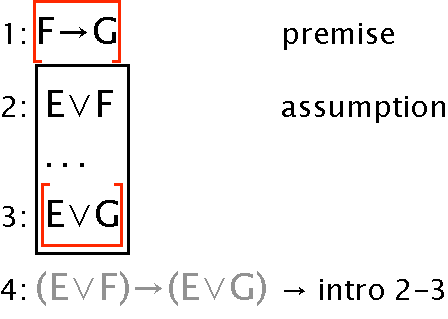
\includegraphics[scale=0.5]{pics/arrowelimhalfbackwardbefore}}}}
\qquad
\subfigure[consequent $G$ deduced from new open conclusion $F$]{
  \label{fig:arrowelimhalfbackwardafter}
  \parbox[b]{200pt}{\centering\fbox{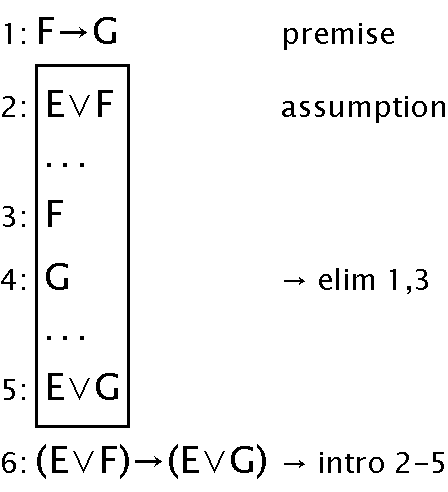
\includegraphics[scale=0.5]{pics/arrowelimhalfbackwardafter}}}}
\caption{$->$ elim half backward, half forward}
\label{fig:arrowelimhalfbackward}
\end{figure}

\section{$->$ steps}

You use $->$ intro backward by selecting a $A->B$ conclusion and then choosing ``$->$ intro'' from the Backward menu. See \figref{arrowintrobackward}, for example. Notice that the step introduces a new assumption and therefore a new box (and that's why it should be used early).

You can use $->$ elim forward by selecting a $A$ hypothesis and a $A->B$ hypothesis, as shown by the trivial example in \figref{arrowelimforward}. (Shift-click to select the second hypothesis: if you select the wrong thing either cancel it with a shift-click or click on the background to cancel all your selections, and start again.)

You can also use $->$ elim half-forward, half-backward if you select a $A->B$ hypothesis and a target conclusion and apply ``$->$ elim'' from the Forward menu. Jape writes a new conclusion $A$ followed by a consequent $B$, as shown in \figref{arrowelimhalfbackward}. It's a half-backward step because it introduces a new conclusion.

$->$ intro forward is just daft, and Jape won't attempt it. $->$ elim backward is possible, but it introduces unknowns and there's no real advantage, so I don't let Jape try.
 
\begin{figure}
\centering
\subfigure[before: conclusion selected]{
  \label{fig:vintrobackwardsiseasyA}
  \parbox[b]{200pt}{\centering\fbox{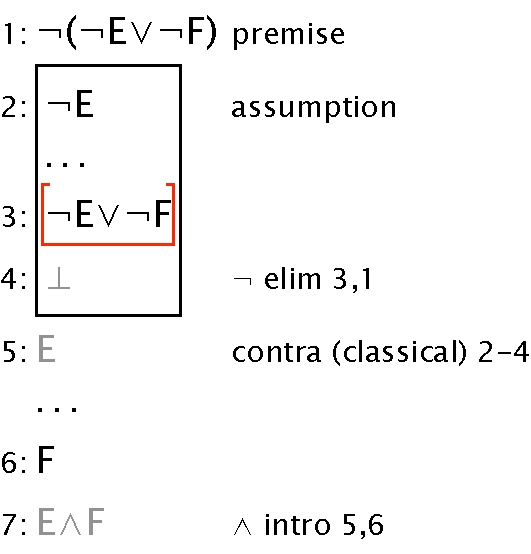
\includegraphics[scale=0.5]{pics/vintrobackwardsiseasyA}}}}
\qquad
\subfigure[after: uncertainty resolved]{
  \label{fig:vintrobackwardsiseasyB}
  \parbox[b]{200pt}{\centering\fbox{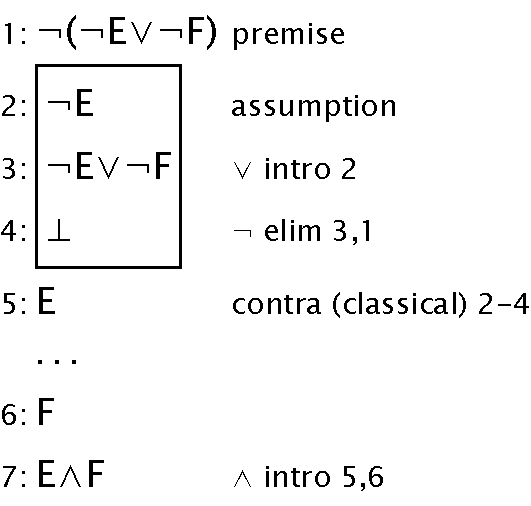
\includegraphics[scale=0.5]{pics/vintrobackwardsiseasyB}}}}
\caption{$|$ intro backwards is easy}
\label{fig:vintrobackwardsiseasy}
\end{figure}

\begin{figure}
\centering
\subfigure[before: hypothesis selected]{
  \label{fig:vintroforwardsgeneratesunknownA}
  \parbox[b]{200pt}{\centering\fbox{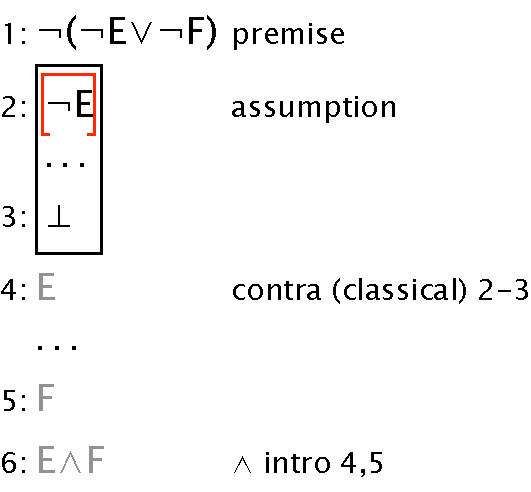
\includegraphics[scale=0.5]{pics/vintroforwardsgeneratesunknownA}}}}
\qquad
\subfigure[after: `unknown' formula introduced]{
  \label{fig:vintroforwardsgeneratesunknownB}
  \parbox[b]{200pt}{\centering\fbox{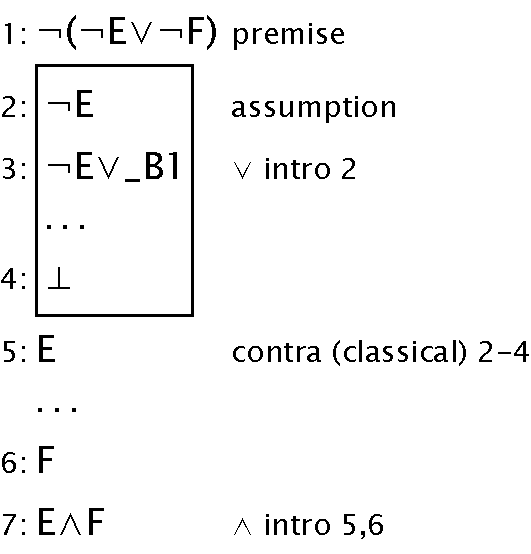
\includegraphics[scale=0.5]{pics/vintroforwardsgeneratesunknownB}}}}
\caption{$|$ intro forwards generates an unknown}
\label{fig:vintroforwardsgeneratesunknown}
\end{figure}

\section{$|$ steps}

Because $|$ elim forwards implements argument by cases, and because the consequent $C$ can't be deduced from the $A|B$ antecedent, it generates big proof changes from a small gesture. That frightens novices, but be brave, because $|$ elim is one of the rules that generates assumptions, so you have to use it as early as possible in a proof.

$|$ intro backwards is destructive --- it throws away half a conclusion --- so you use it as \emph{late} as possible, even though it's very easy to use.

You use $|$ elim forwards by selecting a hypothesis which fits $A|B$, an open conclusion $C$ (if there's only one available conclusion, and if its on the line below the hypothesis, Jape will let you off the conclusion selection) and ``$|$ elim'' from the Forward menu. See \figref{velimneedstargetconclusion} on page \pageref{fig:velimneedstargetconclusion}, for example. Note that the boxes representing the $A$ leads to $C$ and $B$ leads to $C$ arguments (lines 7-8 and 9-10 in \figref{velimneedstargetconclusionbefore}, for example) are written just above the selected conclusion $C$, and the justification is (of course) written against the selected conclusion.

$|$ intro is easy to use backwards: select an open conclusion, decide which half to keep and which to throw away, and apply the corresponding step (``$|$ intro (preserving left)'' or ``$|$ intro (preserving right)'') from the Backward menu. See \figref{vintrobackwardsiseasy}, for example.

For some reason that I've forgotten, I was persuaded to allow $|$ intro forward. I rather regret it, because this isn't a step for novices to use. But, if you must: you select a hypothesis, decide which half of the consequent it has to be, and apply the corresponding step (``$|$ intro (inventing left)'' or ``$|$ intro (inventing right)'') from the Forward menu. The step always invents an unknown, as illustrated in \figref{vintroforwardsgeneratesunknown} by an ``inventing right'' step, and you have to deal with the unknown somehow (see \chapref{unknowns} for suggestions).

If unknowns frighten you, don't use $|$ intro forwards (the easy way to solve the proof problem in \figref{vintroforwardsgeneratesunknown}, for example, is $!$ elim forwards from line 1 with target conclusion line 4, producing \figref{vintrobackwardsiseasyA}; then $|$ intro backwards preserving left produces \figref{vintrobackwardsiseasyB}). 

$|$ elim backwards would be possible, but not for novices, so I didn't allow it.

\begin{figure}
\centering
\subfigure[before: hypothesis $!(E|F)$ and target conclusion selected]{
  \label{fig:!elimforwardsiseasyA}
  \parbox[b]{200pt}{\centering\fbox{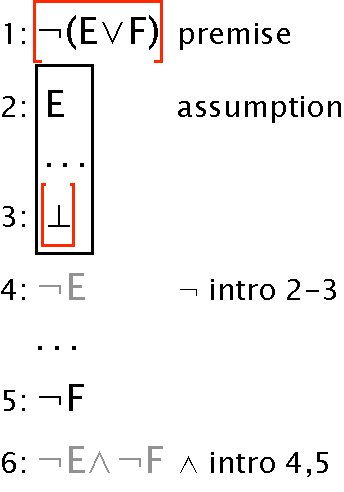
\includegraphics[scale=0.5]{pics/!elimforwardsiseasyA}}}}
\qquad
\subfigure[after: conclusion $E|F$ generated]{
  \label{fig:!elimforwardsiseasyB}
  \parbox[b]{200pt}{\centering\fbox{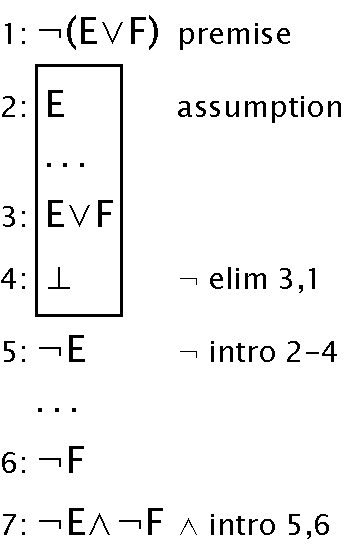
\includegraphics[scale=0.5]{pics/!elimforwardsiseasyB}}}}
\caption{$!$ elim forwards is easy}
\label{fig:!elimforwardsiseasy}
\end{figure}

\begin{figure}
\centering
\subfigure[before: conclusion $!F$ selected]{
  \label{fig:!introbackwardsiseasyA}
  \parbox[b]{200pt}{\centering\fbox{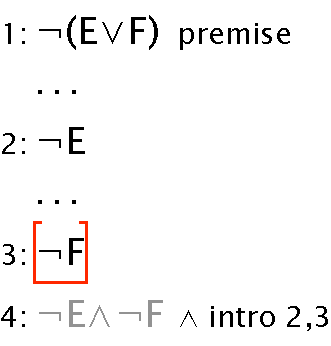
\includegraphics[scale=0.5]{pics/!introbackwardsiseasyA}}}}
\qquad
\subfigure[after: contradiction argument outlined]{
  \label{fig:!introbackwardsiseasyB}
  \parbox[b]{200pt}{\centering\fbox{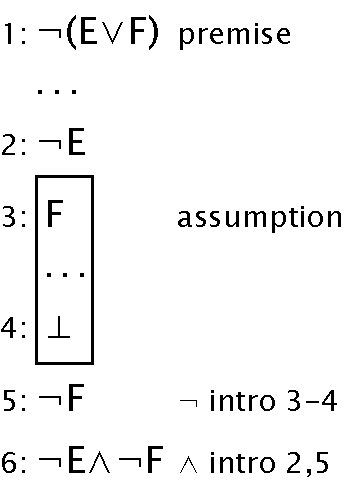
\includegraphics[scale=0.5]{pics/!introbackwardsiseasyB}}}}
\caption{$!$ intro backwards is very easy}
\label{fig:!introbackwardsiseasy}
\end{figure}

\begin{figure}
\centering
\subfigure[before: conclusion $\bot$ selected]{
  \label{fig:!elimbackwardsisharderA}
  \parbox[b]{200pt}{\centering\fbox{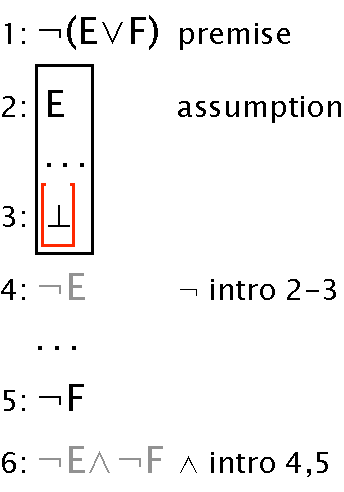
\includegraphics[scale=0.5]{pics/!elimbackwardsisharderA}}}}
\qquad
\subfigure[after: unknown $\_\mathit{B1}$ invented, and two conclusions generated]{
  \label{fig:!elimbackwardsisharderB}
  \parbox[b]{200pt}{\centering\fbox{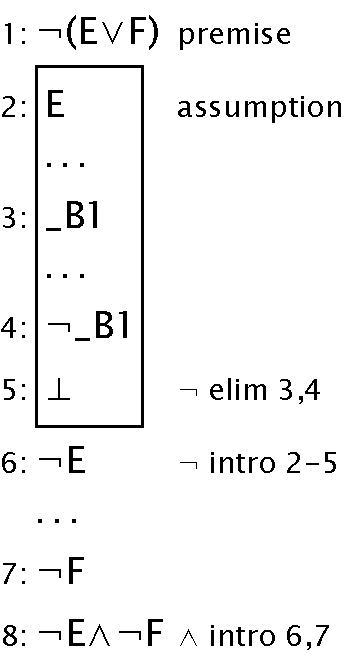
\includegraphics[scale=0.5]{pics/!elimbackwardsisharderB}}}}
\caption{$!$ elim backwards is harder}
\label{fig:!elimbackwardsisharder}
\end{figure}

\section{$!$ steps}

$!$ elim works best forwards, $!$ intro backwards.

To use $!$ elim forwards, select a hypothesis $!A$, or two hypotheses $!A$ and $A$, and choose ``$!$ elim'' from the Forward menu. You can select a target conclusion too, if you like. The step generates a consequent $\bot$, (plus a conclusion $A$  if you only select one hypothesis). See \figref{!elimforwardsiseasy}, for example.

To use $!$ intro backwards, select an open conclusion $!B$ and ``$!$ intro'' from the Backward menu. See \figref{!introbackwardsiseasy}, for example.

It's possible to use $!$ elim backwards, if you select an open conclusion $\bot$. It generates an unknown $\_B$ and two new open conclusions $!\_B$ and $!\_B$, as illustrated in \figref{!elimbackwardsisharder}. It's usually easier to do it forwards, though.

$!$ intro forwards doesn't make much sense, so I didn't allow it.

\begin{figure}
\centering
\subfigure[before: conclusion $E|!E$ selected]{
  \label{fig:classicalcontrastepA}
  \parbox[b]{200pt}{\centering\fbox{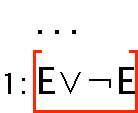
\includegraphics[scale=0.5]{pics/classicalcontrastepA}}}}
\qquad
\subfigure[after: contradiction argument outlined]{
  \label{fig:classicalcontrastepB}
  \parbox[b]{200pt}{\centering\fbox{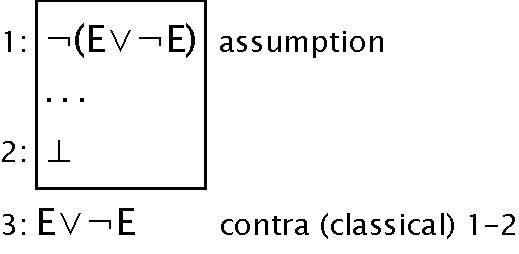
\includegraphics[scale=0.5]{pics/classicalcontrastepB}}}}
\caption{A sample classical contradiction step}
\label{fig:classicalcontrastep}
\end{figure}

\begin{figure}
\centering
\subfigure[before: hypothesis $\bot$ and target conclusion selected]{
  \label{fig:constructivecontraforwardsA}
  \parbox[b]{200pt}{\centering\fbox{\includegraphics[scale=0.5]{pics/constructivecontraforwardsA}}}}
\qquad
\subfigure[after: conclusion `proved']{
  \label{fig:constructivecontraforwardsB}
  \parbox[b]{200pt}{\centering\fbox{\includegraphics[scale=0.5]{pics/constructivecontraforwardsB}}}}
\caption{A sample constructive contradiction step}
\label{fig:constructivecontraforwards}
\end{figure}

\section{$\bot$ (contradiction) steps}

Classical contra is a hard rule to use (there ought to be a blues song about that), but you know you are going to have to use it for some problems. It only works backwards. Constructive contra is easier if you use it forwards.

To use classical contra, select an open conclusion $A$ and choose ``contra (classical)'' from the Backward menu. It creates a hypothetical contradiction argument with assumption $!A$, as shown in \figref{classicalcontrastep}.

To use constructive contra forwards, select a $\bot$ hypothesis and an open conclusion, and choose ``contra (constructive)'' from the Forward menu. See \figref{constructivecontraforwards}, for example.

Constructive contra backwards is destructive: it throws away whatever conclusion it is applied to. But you can do it if you want to. Classical contra forwards would be absurd.

\section{$\top$ (truth) step}

You can always prove $\top$ as an open conclusion: select it and apply ``truth'' from the Backward menu. And that's all you can do with $\top$: no forward step is possible.

\begin{figure}
\centering
\subfigure[before: $@*x.!R(x)$ conclusion selected]{
  \label{fig:forallintrobackwardsA}
  \parbox[b]{200pt}{\centering\fbox{\includegraphics[scale=0.5]{pics/forallintrobackwardsA}}}}
\qquad
\subfigure[after: generalised proof outline introduced, with private variable $i$]{
  \label{fig:forallintrobackwardsB}
  \parbox[b]{200pt}{\centering\fbox{\includegraphics[scale=0.5]{pics/forallintrobackwardsB}}}}
\caption{A $@*$ intro step backwards}
\label{fig:forallintrobackwards}
\end{figure}

\begin{figure}
\centering
\subfigure[before: $@*x.(R(x)@S(x))$ and $\protect\<actual> i$ hypotheses selected]{
  \label{fig:forallelimforwardsA}
  \parbox[b]{200pt}{\centering\fbox{\includegraphics[scale=0.5]{pics/forallelimforwardsA}}}}
\qquad
\subfigure[after: $R(i)@S(i)$ consequent deduced]{
  \label{fig:forallelimforwardsB}
  \parbox[b]{200pt}{\centering\fbox{\includegraphics[scale=0.5]{pics/forallelimforwardsB}}}}
\caption{A $@*$ elim step forwards}
\label{fig:forallelimforwards}
\end{figure}

\section{$@*$ steps}
\var{i1,i2}
$@*$ intro works backwards, $@*$ elim forwards. $@*$ intro is worth using early, because it introduces a variable. The privacy condition on the $@*$ intro step won't usually bother you, because Jape always invents a new variable ($i$, $\<i1>$, $\<i2>$, and so on).

To use $@*$ intro backwards, select an open conclusion $@*x.P(x)$ and choose ``$@*$ intro'' from the Backward menu. Jape builds the outline of the generalised proof, as illustrated in \figref{forallintrobackwards}. 

To use $@*$ elim forwards, you must select a hypothesis $@*x.P(x)$ and also $\<actual> j$, then choose ``$@*$ elim'' from the Forward menu. The effect is illustrated in \figref{forallelimforwards}.

%If your proof attempt contains unknowns then $@*$ intro may generate provisos: see \secref{provisos}.

\begin{figure}
\centering
\subfigure[before: $|*x.!R(x)$ hypothesis and target conclusion $\bot$ selected]{
  \label{fig:existselimforwardsA}
  \parbox[b]{200pt}{\centering\fbox{\includegraphics[scale=0.5]{pics/existselimforwardsA}}}}
\qquad
\subfigure[after: generalised proof outline introduced, with private variable $i$]{
  \label{fig:existselimforwardsB}
  \parbox[b]{200pt}{\centering\fbox{\includegraphics[scale=0.5]{pics/existselimforwardsB}}}}
\caption{An $|*$ elim step forwards}
\label{fig:existselimforwards}
\end{figure}

\begin{figure}
\centering
\subfigure[before: $|*x.!R(x)$ conclusion and $\protect\<actual> i$ hypothesis selected]{
  \label{fig:existsintrobackwardsA}
  \parbox[b]{200pt}{\centering\fbox{\includegraphics[scale=0.5]{pics/existsintrobackwardsA}}}}
\qquad
\subfigure[after: $!R(i)$ antecedent deduced]{
  \label{fig:existsintrobackwardsB}
  \parbox[b]{200pt}{\centering\fbox{\includegraphics[scale=0.5]{pics/existsintrobackwardsB}}}}
\caption{An $|*$ intro step backwards}
\label{fig:existsintrobackwards}
\end{figure}

\section{$|*$ steps}
$|*$ intro works backwards, $|*$ elim forwards. $|*$ elim is worth using early, because it introduces a variable. The privacy condition on the $|*$ elim step won't usually bother you, because Jape always invents a new variable ($i$, $\<i1>$, $\<i2>$, and so on).

To use $|*$ elim forwards, you must select a hypothesis $|*x.P(x)$ and also a target conclusion, and then choose ``$|*$ elim'' from the Forward menu. The justification is written next to the target conclusion, and a generalised proof outline is introduced, as illustrated in \figref{existselimforwards}.

To use $|*$ intro backwards, you must select a conclusion $|*x.P(x)$ and also a hypothesis $\<actual> j$, and then choose ``$|*$ intro'' from the Backward menu. The effect is illustrated in \figref{existsintrobackwards}.

%If your proof attempt contains unknowns then $|*$ elim may generate provisos: see \secref{provisos}.

\chapter{Unknowns, hyp and Unify}
\label{chap:unknowns}
\var{B1}

When James Aczel looked at novices learning logic with Jape, he pointed out that they found \emph{incomplete steps} quite disconcerting. Incomplete steps are ones that let you leave out important information so that you can fill it in later, when you've discovered what it ought to be. You might be allowed to leave out the variable in an $|*$ intro step, for example, and fill it in later. 

Jape uses \emph{unknowns} --- names starting with an underscore, like $\_\<B1>$ --- to stand for formulae which can be filled in later. Even though James persuaded me to eliminate almost all incomplete steps from my treatment of natural deduction, my users pleaded with me to allow some. So it is possible to introduce unknowns into a Jape proof, and because of that it's necessary to know how to get rid of them again.

To understand what follows you have to recognise the distinction between \emph{formula selection} (red box round a conclusion or a hypothesis formula) and \emph{subformula selection} (yellow background behind part or all of a conclusion or hypothesis formula). Note, in particular, that a subformula selection that encompasses a complete formula is \emph{not} the same thing as a formula selection.

\begin{figure}
\centering
\subfigure[before: $|*x.!R(x)$ hypothesis selected]{
  \label{fig:orintroforwardsA}
  \parbox[b]{200pt}{\centering\fbox{\includegraphics[scale=0.5]{pics/orintroforwardsA}}}}
\qquad
\subfigure[after: unknown $\_\protect\<B1>$ introduced in consequent]{
  \label{fig:orintroforwardsB}
  \parbox[b]{200pt}{\centering\fbox{\includegraphics[scale=0.5]{pics/orintroforwardsB}}}}
\caption{An $|$ intro step forwards}
\label{fig:orintroforwards}
\end{figure}

\begin{figure}
\centering
\subfigure[before: conclusion is $\bot$]{
  \label{fig:notelimbackwardsA}
  \parbox[b]{200pt}{\centering\fbox{\includegraphics[scale=0.5]{pics/notelimbackwardsA}}}}
\qquad
\subfigure[after: unknown $\_\protect\<B1>$ introduced in antecedents]{
  \label{fig:notelimbackwardsB}
  \parbox[b]{200pt}{\centering\fbox{\includegraphics[scale=0.5]{pics/notelimbackwardsB}}}}
\caption{A $!$ elim step backwards}
\label{fig:notelimbackwards}
\end{figure}

\section{Introducing an unknown}

$|$ elim backwards takes a formula with an $|$ connective and throws away half of it, because from $A$ you can prove $A|B$, and from $B$ you can prove $A|B$. Some obsessively-forward reasoners wanted me to allow $|$ intro forwards, and just to spite them I did: it's there in the Forward menu, under the line. \Figref{orintroforwards} shows how you can deduce $A|\_B$ from $A$ by choosing ``$|$ intro (inventing right)'' from the Forward menu.

$!$ elim backwards is another good way to get an unknown, illustrated in \figref{notelimbackwards}. There's only one unknown in the proof, but it occurs twice.

These are by no means the only way to introduce unknowns into a proof. One very interesting way is to select a conclusion, choose ``Text command'' from the File menu, type ``apply cut'' and press return. You will get an unknown, intermediate between the hypotheses and your conclusion. I leave you to work out how useful that can be.

\begin{figure}
\centering
\subfigure[before: conclusion $\bot$ selected, subformula $!R(x)$ selected]{
  \label{fig:notelimbackwardswithsubformulaA}
  \parbox[b]{200pt}{\centering\fbox{\includegraphics[scale=0.5]{pics/notelimbackwardswithsubformulaA}}}}
\qquad
\subfigure[after: $!R(x)$ used in antecedents of $!$ elim]{
  \label{fig:notelimbackwardswithsubformulaB}
  \parbox[b]{200pt}{\centering\fbox{\includegraphics[scale=0.5]{pics/notelimbackwardswithsubformulaB}}}}
\caption{A $!$ elim step backwards with subformula selection}
\label{fig:notelimbackwardswithsubformula}
\end{figure}

\section{Avoiding unknowns by subformula selection}

If you know beforehand what should go in place of the unknown, you can tell Jape what to use at the time you make an $|$ intro or $!$ elim step, by subformula selection (alt/option/middle-press-and-drag over the formula or subformula you want to use). \Figref{notelimbackwardswithsubformula} shows an example: note that the hypothesis is \emph{not} selected, but $!R(x)$ is subformula-selected.

\begin{figure}
\centering
\subfigure[before: subformulae $|*x.!R(x)$ and $\_\protect\<B1>$ selected]{
  \label{fig:unifyreplacesunknownA}
  \parbox[b]{200pt}{\centering\fbox{\includegraphics[scale=0.5]{pics/unifyreplacesunknownA}}}}
\qquad
\subfigure[after: instances of $\_\protect\<B1>$ replaced by $|*x.!R(x)$]{
  \label{fig:unifyreplacesunknownB}
  \parbox[b]{200pt}{\centering\fbox{\includegraphics[scale=0.5]{pics/unifyreplacesunknownB}}}}
\caption{Effect of a Unify command}
\label{fig:unifyreplacesunknown}
\end{figure}

\section{Eliminating an unknown with Unify}

If you have an unknown in your proof, and a subformula somewhere in the proof which you want to use to replace the unknown, then subformula selection and the ``Unify'' command from the Edit menu will do the job. You subformula-select two or more subformulae which you want to make the same by replacing unknowns (command/control-alt/option/middle-press-and-drag is the gesture you need to make more than one subformula selection). \Figref{unifyreplacesunknown} shows an example. Note that there are no formula selections in \figref{unifyreplacesunknownA}, only subformula selections.

\begin{figure}
\centering
\subfigure[before: hypothesis $!|*x.!R(x)$ and conclusion $!\_\protect\<B1>$ selected]{
  \label{fig:hypreplacesunknownA}
  \parbox[b]{200pt}{\centering\fbox{\includegraphics[scale=0.5]{pics/hypreplacesunknownA}}}}
\qquad
\subfigure[after: instances of $\_\protect\<B1>$ replaced by $|*x.!R(x)$]{
  \label{fig:hypreplacesunknownB}
  \parbox[b]{200pt}{\centering\fbox{\includegraphics[scale=0.5]{pics/hypreplacesunknownB}}}}
\caption{Effect of \texttt{hyp} on an unknown}
\label{fig:hypreplacesunknown}
\end{figure}

\section{Eliminating an unknown with \texttt{hyp}}

The \texttt{hyp} step is really just a cloak for the Unify command: make this selected conclusion the same as this selected hypothesis (or these selected hypotheses). For example see \figref{hypreplacesunknown}. Note that making $!|*x.!R(x)$ the same as $!\_\<B1>$ means making $|*x.!R(x)$ the same as $\_\<B1>$.

\begin{figure}
\centering
\parbox[b]{250pt}{\centering\includegraphics[scale=0.5]{pics/proofwithproviso}
\caption{Proof with proviso}
\label{fig:proofwithproviso}}
\quad
\parbox[b]{200pt}{\centering\fbox{\includegraphics[scale=0.5]{pics/disallowedunification}}
\caption{Preparation for proviso-violating unification}
\label{fig:disallowedunification}}
\end{figure}

\begin{figure}
\centering
\includegraphics[scale=0.45]{pics/NOTINerrormessage}
\caption{Jape's reason for rejecting unification step}
\label{fig:NOTINerrormessage}
\end{figure}

\section{Provisos and the privacy condition}
\label{sec:provisos}

Recall that the $@*$ intro and $|*$ elim steps introduce a variable --- $i$, $\<i1>$, $\<i2>$, ... --- for private use within a generalised proof. If a proof attempt doesn't include unknowns, Jape can enforce the privacy condition easily: simply use a variable that isn't in use already, anywhere in the proof. If there are unknowns about, things aren't so simple: Jape has to ensure that you don't unify that unknown with a formula that uses the private variable, because that could violate the privacy condition. 

\Figref{proofwithproviso} shows what happens when Jape has to invent a variable and there is an unknown in the proof. It must prohibit the possibility that the formula $\_\<B1>$ includes the variable $i$: it does this with the \emph{proviso} ``$i \text{ NOTIN } \_\<B1>$'' in the \emph{proviso pane} below the proof. \Figref{disallowedunification} shows preparation for an attempt to violate the proviso with a Unify command (making $\_\<B1>$, which appears outside the box, the same as $R(i)$ inside the box). \Figref{NOTINerrormessage} shows the error message that Jape generates when you try the unification.

You get the same situation if you try the steps in the other order ($@*$ intro backwards, $|$ intro forwards selecting only the hypothesis).


\chapter{Disproof}
\label{chap:disproof}

My encoding of natural deduction in Jape deals with disproof by allowing you to make Kripke diagrams which Jape will check against a sequent to see if they are examples, or counter-examples, or neither. You do it by manipulating blobs, lines and atomic formulae in a \emph{disproof pane} above the proof.

Jape shows you what is going on by underlining and colouring formulae and subformulae in the sequent and by colouring blobs on the screen. This chapter should, therefore, be read in colour rather than in monochrome.\footnote{I am aware that use of colour means that some people can't use Jape as easily as others. This is only the tip of a nasty iceberg: Jape uses a visual presentation to make it easier to understand proof and disproof, and that excludes many people with reduced visual acuity from using it at all.

Contrary to some propaganda, these problems aren't easy to overcome. But I'd love to try, and I'd love to hear from anybody who has suggestions to make, advice to offer, technical information to share, guinea-piggery to volunteer, whatever. Messages to me at the title page address, as usual.}

\begin{figure}
\centering
\includegraphics[scale=0.5]{pics/disproofpane}
\caption{Proof attempt with proof pane below and disproof pane above}
\label{fig:disproofpane}
\end{figure}

\section{Getting started}

At any point during a proof attempt you can invoke `Disprove' from the Edit menu.\footnote{There isn't a Disprove button in the conjecture panels. Perhaps there should be! You have to hit Prove to start a proof attempt and then choose Edit:Disprove.} Jape splits the proof window and shows you a Kripke diagram with a single empty world and the proof-attempt sequent (you can select hypotheses and conclusions to construct an alternative sequent: see below) in a \emph{disproof pane} above the proof pane. The sequent may already be underlined and coloured as in \figref{disproofpane}.

The main things to notice in this illustration are
\begin{itemize}
\item the blob in the diagram is ringed in \textcolor{red}{red};
\item some of the names and connectives in the sequent are coloured \textcolor{magenta}{magenta}, some are \textcolor{halfgrey}{grey}, and some are black;
\item some of the formulae are \textcolor{magenta}{\underline{underlined}} and some are not;
\item the sequent uses the semantic turnstile $|=$; 
\item there's a little green waste bin on the right;
\item above the waste bin there are some tiles, each containing an atomic formula.
\end{itemize}

In general \textcolor{magenta}{magenta} means `forced', black means `unforced' and \textcolor{halfgrey}{grey} means `irrelevant'.

Because of operating system variations, your window may not look exactly like the illustration, but it will have the same parts. In other illustrations I show the important bits of the proof and/or disproof panes, without the waste bin and the scroll bars and stuff.

\section{Alternative sequents}

If you select a conclusion in the proof pane (or, if Jape doesn't want to let you do that, the reason next to the conclusion) and then hit Edit:Disprove, Jape will use the disproof sequent consisting of the conclusion as consequent and all the hypotheses above it as antecedent formulae. If you select some of the hypotheses as well as the conclusion, they will be used as the antecedents.

You can choose a new disproof sequent at any time, even in the middle of a disproof attempt.

If you want to set up an entirely new challenge, enter it into one of the conjectures panels (New button), hit Prove and then Edit:Disprove in the proof window.

\subsection{Selecting a situation}

\begin{figure}
\centering
\parbox{200pt}{\centering
\includegraphics[scale=0.5]{pics/firstmultiworld}
\caption{A multi-world situation}
\label{fig:firstmultiworld}
}
\qquad
\parbox{200pt}{\centering
\includegraphics[scale=0.5]{pics/parvainmultum}
\caption{A single-world situation}
\label{fig:parvainmultum}
}
\end{figure}

There is always one selected world in a diagram, ringed in \textcolor{red}{red}. The selected world is the root world of the situation evaluated by Jape. For example, in \figref{firstmultiworld} the situation is the whole diagram; in \figref{parvainmultum} it's the single world at top left.

\subsection{What's forced ? --- colouring, greying, underlining}

Jape evaluates all the formulae and sub-formulae of the sequent in the situation with the selected world as its root, and colours all those formulae and sub-formulae. 
\begin{itemize}
\item The default colour is black, and it means \emph{not forced}.
\item If a (sub-)formula's value is never called on --- usually this is true of quantified predicates, for example --- then it's \textcolor{halfgrey}{grey}, meaning \emph{strictly irrrelevant}.
\item An atomic (sub-)formula which is \emph{forced} is coloured \textcolor{magenta}{magenta} (this covers atoms like $E$, atomic predicates like $S(j)$ and individuals like $\<actual> k$).
\item When a non-atomic (sub-)formula is forced, its connective is coloured \textcolor{magenta}{magenta}. 
\item When an entire sequent premise or conclusion is forced, it is \textcolor{magenta}{\underline{underlined}} in \textcolor{magenta}{magenta}.
\end{itemize}
So: when all the premises are magenta-underlined and the conclusion is not, you have a counter-example; when everything is underlined you have an example; otherwise you have nothing in particular.

\begin{figure}
\centering
\parbox{150pt}{\centering
\includegraphics[scale=0.5]{pics/firstcounterexample}
\caption{A simple counter-example}
\label{fig:firstcounterexample}
}
\qquad
\parbox{250pt}{\centering
\includegraphics[scale=0.5]{pics/elaboratecounterexample}
\caption{An elaborate counter-example}
\label{fig:elaboratecounterexample}
}
\end{figure}

\Figref{firstcounterexample} shows a sample counter-example, and the colouring gives a hint of why it's a counter-example: $E$ isn't forced anywhere, so the premise implication is forced (magenta arrow, underlining); and then, because $E->F$ is forced but $G$ isn't, the conclusion isn't forced (black arrow, no underlining). \Figref{elaboratecounterexample} shows an elaborate counter-example: the premises are obviously forced, but there are no individuals to force the $|*$ quantification in the conclusion.

The disproof pane in \figref{disproofpane} shows neither a counter-example nor an example. The premises aren't forced because, as atomic formulae, they aren't present at the root world; the conclusion is forced because every individual in the situation (there aren't any ... remember the green sheep) forces a version of $R(x)->S(x)$. Similar remarks apply to figures \ref{fig:firstmultiworld} and \ref{fig:parvainmultum}.

\section{Making diagrams}

To begin your disproof Jape presents you with the simplest diagram: the isolated empty world. You add components to your diagram --- worlds, formulae and lines --- using drag-and-drop mouse gestures. You can delete components by dragging them to the waste bin. You can add tiles with double-clicks. You can Undo your actions to any degree that you like, and Redo likewise.\footnote{Undo and Redo apply to the last pane you used the mouse in, either proof or disproof.} 

To \emph{move} a component of a diagram you put the mouse pointer over it, press (left button on a multi-button mouse), hold a moment, then --- still pressing --- move to a new position, and finally release. Jape shows you a transparent image of the thing you are dragging, so you can see what you are doing.

To \emph{duplicate} a component you hold down the alt/option key throughout the gesture (or use the middle button on a multi-button mouse) and you drag a new copy of the thing you pressed on.

Sometimes the purpose of the drag is to \emph{drop} one component onto, or into, another. You drag the first component until the mouse pointer is over the one you want to drop onto/into. The recipient will change colour if it's prepared to accept the drop, and you simply let go while it's lit up. If the drop fails (you aren't over a component, or it won't light up) then the dropped component flies back to base.

\subsection{Dragging worlds}

You can move-drag worlds about the place to make your diagram look nicer. You press on the blob, and you drag the blob plus any formulae attached to it. Lines connected to the world stay connected, and you can drop it anywhere you like. To preserve the `connections only upwards' principle, Jape will delete a line if you drag a world below its parent.

By duplicate-dragging a blob, you drag a copy of the world --- the blob plus any formulae attached to it --- with a line attaching it to the world it came from. The new world stays where you put it. If it's above the world you dragged it from, they will be connected by a line. If it's level or below, then no line.

You can drag a world onto a line (which lights up to show you are over it) or another world (which lights up ditto) and Jape does the obvious thing, adding whatever formulae are necessary to whatever worlds in order to maintain monotonicity.

If you drag a world to the waste bin it's deleted, along with all the formulae attached to it and all the lines connected to it. The bin lights up when it will accept the world; it won't accept the currently-selected world.

If you drop the world onto another the two worlds are merged. Jape does the correct monotonicity adjustments to the diagram by adding formulae to the children of the destination.

\subsection{Dragging lines}

You can drag lines and drop them onto worlds or into the waste bin, as you wish. Jape does the obvious thing in each case (if you can't guess what that is, just try it!).

If you want to make a line between world A and world B, where A is below B, duplicate-drag A to B and drop the new world onto B. Jape makes the monotonicity adjustments, adding formulae to B and its children as necessary. Dragging from B to A will have some not-very-useful effect (but there's always Undo!).

\subsection{Dragging formulae}

You can drop a formula on a world, or drag it away from a world, in one of several ways. If a formula is added to a world then, to preserve monotonicity, it is added to the children of that world as well. If a formula is deleted from a world then it is deleted from all ancestors of that world.

You can drag a formula from a tile and drop it onto a world (the world lights up, of course, to show that it's eager to accept; worlds won't accept a second copy of a formula they already have). The formula isn't deleted from the tile, whichever kind of drag gesture you use, because tiles are infinite sources of formula-copies.

You can move-drag a formula from one world onto another; it is added to the destination world and deleted from the source world. If you duplicate-drag it instead, it is simply added to the destination world.

\section{Making individuals and predicate instances}

If a sequent mentions an individual by including a hypothesis like $\<actual> j$, then there will be a tile for that individual (see figures \ref{fig:disproofpane}, \ref{fig:firstmultiworld}, \ref{fig:parvainmultum} and \ref{fig:elaboratecounterexample}, for example). If there are quantifiers but no individuals you will get a free $\<actual> i$ tile.

\var{i1,j1,k1,i2,j2,k2}
If you need more individuals, double-click any ``$\<actual> ...$'' tile. Jape uses an obvious numbering algorithm to name the new individual --- $\<actual> j$, for example, generates first $\<actual> \<j1>$ then $\<actual> \<j2>$, and so on.\footnote{It would be nicer if it went $i$, $j$, $k$, $\<i1>$, $\<j1>$, $\<k1>$, $\<i2>$, ... One day I'll make it do that.}

If you want to make a new predicate instance, double-click a predicate-instance tile. Jape looks through your tiles for unused individuals and uses them to give you a new one. For example if you have a tile for $S(j)$ and tiles for $\<actual> j$ and $\<actual> \<j1>$, then double-clicking $S(j)$ gets you $S(\<j1>)$, as you might expect. If there's more than one instance that could be made, Jape shows you the alternatives and asks you to choose. If you don't have enough individuals to make a new instance, it tells you so.

\begin{figure}
\centering
\parbox{150pt}{\centering
\includegraphics[scale=0.5]{pics/samuels0}
\caption{A counter-example}
\label{fig:samuels0}
}
\qquad
\parbox{150pt}{\centering
\includegraphics[scale=0.5]{pics/samuels1}
\caption{$!!E$ forced here}
\label{fig:samuels1}
}
\parbox{150pt}{\centering
\includegraphics[scale=0.5]{pics/samuels2}
\caption{$!!E->E$ forced here}
\label{fig:samuels2}
}
\qquad
\parbox{150pt}{\centering
\includegraphics[scale=0.5]{pics/samuels3}
\caption{$!E$ forced here}
\label{fig:samuels3}
}
\parbox{150pt}{\centering
\includegraphics[scale=0.5]{pics/samuels4}
\caption{Multiple forcing}
\label{fig:samuels4}
}
\qquad
\parbox{150pt}{\centering
\includegraphics[scale=0.5]{pics/samuels5}
\caption{Too much forcing}
\label{fig:samuels5}
}
\end{figure}

\section{Exploring reasons}

The hardest thing to explain to a novice is \emph{why} a particular formula is forced in a particular situation. \Figref{samuels0} shows a particularly ludicrous formula and its counter-example, which really needs explanation. Jape provides mechanisms which can be some help.

The colouring of atomic (sub-)formulae and connectives is the first mechanism. But with the negative connectives --- $->$ and $!$ --- and with the quantifiers, we often need a bit more help.

Jape allows you to select (click or left-click) or subformula-select (alt/option/middle-press-and-drag) in the sequent. It will colour magenta all the worlds which force the selected (sub)formula. For example, \figref{samuels1} shows where $!!E$ is forced in the difficult example. Figures \ref{fig:samuels2} and \ref{fig:samuels3} show information about some other subformulae.

If you choose more than one formula, Jape colours the worlds that force them all: see figures \ref{fig:samuels4} and \ref{fig:samuels5}.

\begin{figure}
\centering
\includegraphics[scale=0.5]{pics/quantifiers1}
\caption{Support for a quantifier}
\label{fig:quantifiers1}
\end{figure}

If you choose a quantifier formula in the sequent, Jape colours magenta not only the worlds which support it, but also the presence markers which support that formula: i.e. individuals at worlds which which generate a forced formula if you instantiate the quantified formula with them. In \figref{quantifiers1}, for example, worlds which force the selected quantifier are magenta; individuals which support it are magenta too. You can see that $R(k)->R(j)@R(k)$ at each of the worlds in this example.

\section{Completing a disproof}

When you have a disproof (all the premises underlined, the conclusion not underlined), you can register it with Jape using Edit:Done. Disproved conjectures are marked with a cross; proved conjectures get a tick. Because you can prove some conjectures classically and also disprove them constructively, it's possible to get both a tick and a cross together. See \figref{decoratedpanel} on page \pageref{fig:decoratedpanel} for examples.

\section{Printing disproofs}

You can print or export an image of the disproof pane, using Edit:Print Disproof or Edit:Export Disproof.
 
\chapter{Using theorems and stating conjectures}
\label{chap:theorems}

\begin{figure}
\centering
\subfigure[before: conclusion $E|!E$ selected]{
  \label{fig:theorembackwardA}
  \parbox[b]{200pt}{\centering\fbox{\includegraphics[scale=0.5]{pics/theorembackwardA}}}}
\qquad
\subfigure[after: hypothesis $!(!E@!!E)$ generated]{
  \label{fig:theorembackwardB}
  \parbox[b]{200pt}{\centering\fbox{\includegraphics[scale=0.5]{pics/theorembackwardB}}}}
\caption{Theorem applied backward}
\label{fig:theorembackward}
\end{figure}

\section{Using theorems}

A theorem is a proved conjecture, one with a tick next to it in a conjecture panel. Jape lets you use the theorem
\begin{equation*}
A_{1},A_{2},\dots,A_{n}|-B
\end{equation*}
as if it was the rule
\begin{equation*}
\infer{B}
      {A_{1} & A_{2} & \dots & A_{n}}
\end{equation*}
You can apply a theorem backwards  or forwards using the Apply button in its conjecture panel.  

To work backwards, just select an open conclusion in the proof window, select the theorem in its panel, and press the Apply button. Jape will apply the theorem like any rule, instantiating it to fit the conclusion, making antecedents of its premises and entering them as hypotheses or linking to existing hypotheses if possible. See \figref{theorembackward}, for example.

\begin{figure}
\centering
\subfigure[before: hypothesis $(E->F)->E$ selected]{
  \label{fig:singlepremisetheoremforwardA}
  \parbox[b]{200pt}{\centering\fbox{\includegraphics[scale=0.5]{pics/singlepremisetheoremforwardA}}}}
\qquad
\subfigure[after: consequent $(E@F)->E$ generated]{
  \label{fig:singlepremisetheoremforwardB}
  \parbox[b]{200pt}{\centering\fbox{\includegraphics[scale=0.5]{pics/singlepremisetheoremforwardB}}}}
\caption{Single-premise theorem applied forward}
\label{fig:singlepremisetheoremforward}
\end{figure}

\begin{figure}
\centering
\subfigure[before: conclusion selected]{
  \label{fig:nopremisetheoremforwardA}
  \parbox[b]{200pt}{\centering\fbox{\includegraphics[scale=0.5]{pics/nopremisetheoremforwardA}}}}
\qquad
\subfigure[after: theorem inserted, with unknowns]{
  \label{fig:nopremisetheoremforwardB}
  \parbox[b]{200pt}{\centering\fbox{\includegraphics[scale=0.5]{pics/nopremisetheoremforwardB}}}}
\caption{Theorem applied to non-matching conclusion}
\label{fig:nopremisetheoremforward}
\end{figure}

Because forward steps take a lot of careful use of behind-the-scenes technology, theorems work best backwards. But sometimes you must work forwards, and you can do that in two ways.

If your theorem has exactly one premise, you can select a hypothesis to match that premise and apply the theorem like a forward rule, as illustrated in \figref{singlepremisetheoremforward}.

If your theorem has no premises or more than one premise, don't select a hypothesis but do select a conclusion and apply the theorem. It sounds daft but it works: Jape makes a version of the theorem in which all the variable and formula names are replaced by unknowns and inserts it into the proof, as illustrated in \figref{nopremisetheoremforward}. You have to get rid of the unknowns using \texttt{hyp} steps or the Unify command, as described in \chapref{unknowns}.

\begin{figure}
\centering
\includegraphics[scale=0.5]{pics/newconjecturewindow}
\caption{The New Conjecture window}
\label{fig:newconjecturewindow}
\end{figure}

\section{Stating your own conjectures}

Press the ``New...'' button on any conjectures panel and you see a window like \figref{newconjecturewindow}. You type your conjecture using the keyboard in the normal way, and you can use the buttons provided to get the fancy symbols that aren't on your keyboard.

Names in a conjecture have to obey certain rules:
\begin{itemize}
\item \emph{variables} must start with $x$, $y$, $z$, $i$, $j$ or $k$ and can continue with any letter or digit;
\item \emph{formula} or \emph{predicate} names must start with $A$, $B$, $C$, $D$, $E$, $F$, $G$, $H$, $P$, $R$, $S$ or $T$ and can continue with any letter or digit.
\end{itemize}

If you make a mistake, like leaving out a dot or a bracket in a crucial spot, or typing a name it can't recognise, Jape will complain. If you make more than one mistake, Jape only spots the first (reading left to right). Sometimes the error messages will be hard to understand: I'm sorry for that, but it's really hard to improve them. 

\chapter{Troubleshooting}

\section{Problems getting started}

On MacOS / OS X your security settings may stop you running Jape, saying it comes from a unknown developer. There's a way round this: ctrl-click Jape, choose Open from the little menu that appears, and say Open on the alert window that comes up. After that it can be double-clicked as normal.

On Windows and Linux Bernard distributes an `installation jar' -- a bundle of stuff that distributes itself round your filestore. To get Jape and the examples you have to \emph{double-click} it. If asked, open in with java, not jar. Don't unpack it: that doesn't work.

The Jape app can be put anywhere you like. The examples can be anywhere you like. 

If you installed Jape and it won't start properly, throw it all away and install it again. This time follow the instructions \emph{precisely}. Then it will work.

\section{What if a proof step goes wrong?}

When you try to apply a rule one of two things can happen. Either the rule applies, and the step goes through, or it doesn't, and Jape shows you an error message.

Even though a rule does apply and the proof step does go through, it may not turn out to be the right thing to do. Sometimes an apparently successful step can lead to a dead end. Sometimes a step works, but not in the way that you expected --- perhaps lots of unknowns suddenly appear in the proof, or there are lots of extra lines that you didn't expect, or lots of lines suddenly disappear.

Whenever something happens that isn't what you expected, the first stage of a cure is to use the Undo command from the Edit menu. Undo takes you back one step in the proof, two Undos take you back two steps, and so on. Using several Undos can move you back from a dead end to an earlier position from which you can 
move forward in a different direction.

You can even recover from Undo! The Redo command (also in the Edit menu) reverses the effect of Undo, two Redos reverse two Undos, and so on. So if you decide, after Undoing, that you really did want to make the step after all, Redo will make it again. (If you Undo and make a new proof step, then the one you Undid is 
gone for ever, like it or not.)

The Undo command allows you to explore if you don't know what rule or theorem to apply in a proof: you can experiment with different rules and theorems from the menus until you find one that works. That can be a bad thing, if you just try things at random until you find one that happens to work, and don't reflect on what you are doing. It's also the slowest way of finding proofs. But sometimes we all need to search and experiment (aka ``thrash about''), and then Undo and Redo are invaluable. I hope that when you do search and find a surprising avenue that happens to work,. you will pause to ask yourself \emph{why} it works. Jape is designed to support `reflective exploration' --- it helps with the exploring part, and you learn by reflecting on the results.

\end{document}
